\documentclass{article}

% Language setting
% Replace `english' with e.g. `spanish' to change the document language
\usepackage[english, russian]{babel}

% Set page size and margins
% Replace `letterpaper' with `a4paper' for UK/EU standard size
\usepackage[letterpaper,top=2cm,bottom=2cm,left=3cm,right=3cm,marginparwidth=1.75cm]{geometry}

% Useful packages
\usepackage{amsmath}
\usepackage{graphicx}
\graphicspath{ {./theory_images/} }
\usepackage[colorlinks=true, allcolors=blue]{hyperref}
\usepackage[T2A]{fontenc}


\title{Реализация полученных теоретических алгоритмов для задачи о многоруких бандитах с учетом степени отвращения к риску}
\author{Михаил Давыдов}

\begin{document}
\maketitle

\begin{abstract}
В этой статье описываются эксперименты по применению теоретических результатов, полученных в прошлой работе, для задачи о многоруких бандитах с учетом степени отвращения к риску, приводятся обоснования полученных результатов.
\end{abstract}

\section{Введение}

В предыдущей работе были приведены возможные алгоритмы, которые можно применять для аппроксимации оптимального решения для задачи о многоруких бандитах с учетом степени отвращения к риску. В этой статье будут показаны проводимые эксперименты, построены графики для интерпретации результатов. Напомним, если дано $n$ рычагов, и каждый рычаг $i$ соответствует распределению со средним $m_i$ и дисперсией $\sigma_i^2$, то цель -- найти такой вероятностный вектор $\textbf{p}^* \in \Delta^n$, что $\textbf{p}^* = \underset{\textbf{p} \in \Delta^n}{\arg \max} \sum_{i=1}^n p_i m_i - \lambda \sum_{i=1}^n p_i^2 \sigma_i^2$. При этом начальная информация о рычагах неизвестна, и каждый ход, выбирая один из рычагов, мы получаем награду из распределения, соответствующего этому рычагу.

\section{Перенес из теории}

Если параметры распределений известны для нас (но не для алгоритма) в ходе тестирования, то для измерения результата можно использовать 3 метрики. Каждая из наград считается по каждому шагу и усредняется по нескольким сгенерированным различным независимым задачам о многоруких бандитах.
\begin{enumerate}
    \item Ожидаемый портфель $\text{Portf}_t = m_{p_t} - \lambda \sigma_{p_t}^2$. Метрика аналогична награде для обычной задачи о многоруких бандитах. В качестве альтернативы можно использовать сожаление $\text{Regret}_t = \underset{P}{\max} \left( m_p - \lambda \sigma_p^2 \right) - \text{Portf}_t$
    \item Так как мы хотим, чтобы вероятности сошлись к оптимальным как можно быстрее, то можно использовать усредненный по шагам портфель $\overline{\text{Portf}_t} \frac{\sum_{k=1}^t m_{p^k} - \lambda \sigma_{p^k}^2}{t}$ или усредненное сожаление $\overline{\text{Regret}_t} = \underset{P}{\max} \left( m_p - \lambda \sigma_p^2 \right) - \overline{\text{Portf}_t}$.
    \item Пусть вектор вероятностей, при котором достигается макисмальное значение $m_p - \lambda \sigma_p^2$, равен $P = (p^1, ..., p^n)$. Зная $m_i$ и $\sigma_i^2$, его можно получить с помощью метода градиентного подъема (формулой воспользоваться не получится, так как вероятности в нашей задаче неотрицательны). Пусть также полученный вектор вероятностей в задаче о многоруких бандитах равен $B = (b_1, ..., b_n)$. Тогда метрика равна $$\delta = 1 - \frac{1}{2}\sum_{i=1}^n |b_i - p_i|$$
    Заметим, что в обычной задаче о многоруких бандитах $P = (0, ..., 1, 0, ..., 0)$, и новая метрика равна $1 - \frac{1}{2}\left( (1 - b_k) + \sum_{i = 1, i \neq k}^n b_i \right) = 1 - (1 - b_k) = b_k$, то есть совпадает с процентом оптимальных действий, а это есть вторая метрика в обычной задаче о многоруких бандитах. Так как $\delta \in [\underset{i}{\min} (p_i), 1]$, то можно также ввести ``растянутую'' метрику $\hat{\delta} = (\delta - \underset{i}{\min}(p_i) ) \cdot \frac{1}{1 - \underset{i}{\min}(p_i)} \in [0,1]$. Аналогично, можно считать ``сожаление'' и усредненное сожаление.
\end{enumerate}

\section{Проверка greedy-алгоритмов}

\begin{figure}[h] %!t
\centering
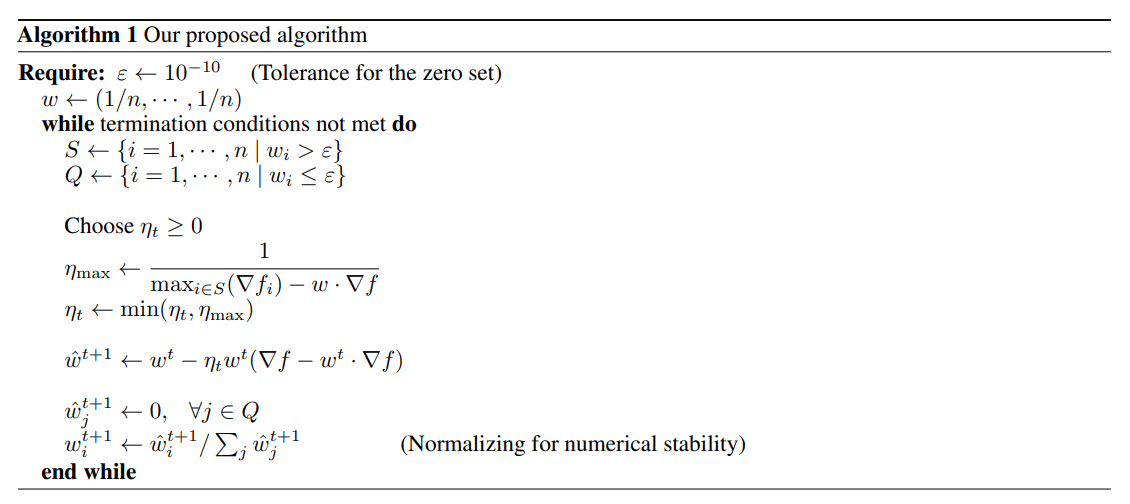
\includegraphics[width=6in]{theory_tester/theory_images/cauchy_simplex.png}
\caption{Псевдокод для алгоритма CauchySimplex}
\label{fig:cauchy_simplex_pseudocode}
\end{figure}

Для начала была проведена проверка 2 алгоритмов для нахождения решения задачи в случае, когда все матожидания и дисперсии известны. Первый алгоритм -- алгоритм нахождения максимума на симплексе, представленный в конце главы ``Стратегии'' (назовем его StandardGreedy). Второй алгоритм -- алгоритм градиентного подъема CauchySimplex, представленный в \cite{cauchy_simplex}. Среди неградиентных методов был рассмотрен только метод StandardGreedy, поскольку он обладает самой меньшим алгоритмической сложностью шага $O(n \log n)$. В CauchySimplex выбраны такие гиперпараметры: $\epsilon = 10^{-3}$, $stop = 10^{-9}$ -- когда изменение $V = \sum_{i=1}^n p_i m_i - \lambda \sum_{i=1}^n p_i^2 \sigma_i^2$ за один шаг меньше, чем $stop$, то алгоритм останавливается (см. \ref{fig:cauchy_simplex_pseudocode}). \\

Далее происходит запуск 500 тестов, в каждом тесте было 10 распределений со средними, выбранными случайно из $\mathcal{N}(1,1)$, и дисперсиями $\sigma^2$, т.ч. $\sigma \sim Exp(2)$.  Чтобы включить среди рычагов ``безрисковые'' рычаги, каждая из дисперсий с вероятностью $\frac{1}{n}$ ($n=10$) домножалось на 0. Для каждого такого набора матожиданий и дисперсий запускались алгоритмы StandardGreedy и CauchySimplex, после чего полученные вероятности сравнивались. Если хотя бы 2 вероятности отличаются больше, чем на гиперпараметр error\_rate, тест считался проваленным. Алгоритм, сравнивающий подходы, был запущен 2 раза для error\_rate$=0.02$ и error\_rate$=0.05$. \\

В результате при error\_rate$=0.02$ количество проваленных тестов равнялось $2.8\%$, а при error\_rate$=0.05$ все тесты прошли успешно (см. \ref{fig:comparison_standard_greedy_cauchy_simplex}). При этом среднее выполнение CauchySimplex составляет от 90 до 160 миллисекунд, в то время как StandardGreedy -- меньше $0.1$ миллисекунды. Это позволяет сделать 3 вывода:
\begin{enumerate}
    \item Ввиду того, что CauchySimplex относится к градиентным методам и потому обладает некоторой погрешностью, и этот алгоритм выдает оптимальное решение, то и алгоритм StandardGreedy выдает оптимальное решение.
    \item Погрешность метода CauchySimplex иногда достаточно большая.
    \item Алгоритм StandardGreedy намного быстрее CauchySimplex.
\end{enumerate}
На основании этого можно сделать вывод, что StandardGreedy более применим для проведения экспериментов.

\begin{figure}[ht!] %!t
\centering
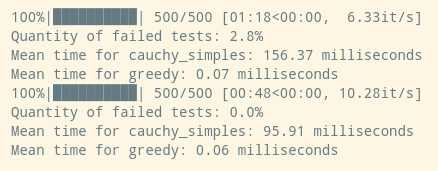
\includegraphics[width=4in]{theory_tester/theory_images/results_compare.png}
\caption{Результаты сравнения алгоритмов CauchySimplex и StandardGreedy}
\label{fig:comparison_standard_greedy_cauchy_simplex}
\end{figure}

\section{Методология}

Для рассмотрения алгоритмов было использовано 10 рычагов. Все рычаги относятся к одному семейству распределений. Было рассмотрено 4 разлтчных семейства распределений: нормальное распределение ($\mathcal{N}(a,\sigma^2)$ или $t_{\infty}$), которое является предельным случаем распределения Стьюдента при числе степеней свободы, стремящемся к бесконечности; распределение Стьюдента с 3 степенями свободы ($t_3$), домноженное на $\frac{1}{\sqrt{3}} \cdot \sigma$, чтобы дисперсия была равна $\sigma^2$ (значение $\sigma^2$ будет введено позже); распределение Стьюдента с $\mu=2.1$ ($t_{2.1}$) домноженное на $\frac{1}{\sqrt{21}} \cdot \sigma$, чтобы дисперсия была равна $\sigma^2$; распределение Стьюдента с 2 степенями свободы $t_2$ домноженное на $\sigma_{\text{scale}}$. Хотя для последнего распределения цель максимизации $\sum_{i=1}^n p_i m_i - \lambda \sum_{i=1}^n p_i^2 \sigma_i^2$ некорректна, поскольку у $t_2$ нет дисперсии, можно вместо дисперсии $\sigma^2$ подставить параметр растяжения $\sigma_{\text{scale}}^2$, возведенный в квадрат, то есть пытаться найти $\sum_{i=1}^n p_i m_i - \lambda \sum_{i=1}^n p_i^2 \sigma_{i, \text{scale}}^2$. Естественно, вся разработанная до этого теория не работает для максимизации измененной величины. \\
Каждое из распределений было смещено на значение, выбранное случайно из $\mathcal{N}(1,1)$, а также домножено на $\sigma \sim Exp(2)$. Чтобы включить среди рычагов ``безрисковые'' рычаги, после домножения на $\sigma$ каждое из распределений с вероятностью $\frac{1}{n}$ ($n=10$) домножалось на 0. Таким образом, с вероятностью примерно $1 - e^{-1} \approx 63\%$ среди рычагов есть хотя бы один с нулевой дисперсией. \\


Изнаально выбирались следующие стратегии:
\begin{enumerate}
    \item $\epsilon$-greedy стратегии, то есть стратегии, действующие по формуле
    $$\textbf{p}_t = \begin{cases}
            \underset{\textbf{p} \in \Delta^n}{\arg \max} \sum_{i=1}^n p_i Q_t(i) - \lambda \sum_{i=1}^n p_i^2 S_t^2(i), & \text{with probability} \; 1 - \epsilon, \\
            (\frac{1}{n}, ..., \frac{1}{n}), & \text{with probability} \; \epsilon.
            \end{cases}$$ 
    Максимум здесь и далее находится с помощью алгоритма StandardGreedy. Далее выбираются $\epsilon$-greedy стратегии с $\epsilon = 0$ (то есть просто жадная стратегия), $0.01, 0.1$. Изначально $\forall a \; Q_t(a) = 0, \: Q_t^2(a) = 0$.
    \item $\epsilon$-greedy стратегии с $\epsilon=0.1$ и скорректированной дисперсией. Об этом подробнее в разделе~\ref{sec:correction_eps_greedy}.
    \item Далее берутся $\epsilon$-greedy стратегии с адаптивным $\epsilon$, то есть меняющимся со временем. Были взяты adaptive $\epsilon$-greedy (когда $\epsilon = \frac{\epsilon_0}{t}$) с $\epsilon_0=1$ и $\epsilon_0=10$ (если $\epsilon > 1$, то берется $\epsilon=1$), и VDBE с $\tau=1, \: \delta=0.1$, примененные к $\epsilon_0=1$ и $\epsilon=10$. Полученные результаты были сравнены с $\epsilon$-greedy стратегией с $\epsilon=0.1$.
    \item Затем были взяты стратегии с оптимистичной инициализацией, то есть стратегии, для которых изначально $\forall a \; Q_t(a) = d, \; d > 0$. В качестве  $d$ был выбран $d=6$. Обновление $Q_t(a)$ происходит с константынм шагом (step-size) в соответствии с материалом \href{https://matteosantama.github.io/ewm/}{на этой странице}. Был выбран step-size$ = 0.1$. Сравниваются greedy-стратегию с оптимистичной инициализацией с $0.1$-greedy стратегиями с обычной и оптимистичной инициализациями.
    \item Upper-Confidence-Bound Action Selection -- вместо $Q_t(a)$ берется верхняя граница доверительного интервала для $Q_t(a)$. Поскольку неравенства Хаффдинга дли дисперсии не существует, а в классическом UCB для обоснования причины, почему в качестве верхней граница доверительного интервала берется $Q_t(a) + c \sqrt{\frac{ln \; t}{N_t(a)}}$, используется именно неравенство Хаффдинга \cite{intro_to_multiarmed}, то подаваемая в StandardGreedy дисперсия не меняется. Итоговая формула выглядит так:
    $$\textbf{p}_t = \underset{\textbf{p} \in \Delta^n}{\arg \max} \; \sum_{i=1}^n p_i \cdot \left[ Q_t(i) + c \sqrt{\frac{ln \; t}{N_t(i)}} \right] - \lambda \sum_{i=1}^n p_i^2 S_t^2(i) ,\; c > 0$$
    То есть вместо $Q_t(a)$ в StandardGreedy подается $Q_t(i) + c \sqrt{\frac{ln \; t}{N_t(i)}}$. В случае, когда $N_t(a) = 0$, подставляется $N_t(a) = 0.001$. UCB с $c = 2$ сравнивается с $0.1$-greedy стратегией.
    \item Gradient bandits: ИСПРАВЬ КОД И НАПИШИ В ИЗМЕНЕННОМ ВИДЕ.
    Я сравнил результаты gradient bandits для $\alpha = 0.1, \; 0.4$, и в случаях, когда baseline есть и когда его нет. При этом моды распределений специально смещены на 4, чтобы показать, что, в отличие от других стратегий gradient bandit невосприимчив к смещению распределений.
\end{enumerate}

Каждая из стратегий была запущена для каждого из распределений на 2000 независимых тестах (для каждого теста свое смещение распределений) длиной 1000 шагов каждый, после чего посчитаны среднее сожаление $\text{Regret} = \left( \sum_{i=1}^n p_i^* Q_t(i) - \lambda \sum_{i=1}^n (p_i^*)^2 S_t^2(i) \right) - \left( \sum_{i=1}^n p_i Q_t(i) - \lambda \sum_{i=1}^n (p_i)^2 S_t^2(i) \right)$, среднее реальное сожаление $\text{Regret}_{\text{real}} = \left( \sum_{i=1}^n p_i^* m_i - \lambda \sum_{i=1}^n (p_i^*)^2 \sigma_i^2 \right) - \left( \sum_{i=1}^n p_i m_i - \lambda \sum_{i=1}^n (p_i)^2 \sigma_i^2 \right)$ и процент выбранных оптимальных действий на каждом шаге $Opt = 1 - 2 \sum_{i=1}^n |p_i - p_i^*|$, где $\textbf{p}^*$ -- решение исходной задачи. Для каждого распределения и каждой метрики результаты для одной группы стратегий визуализированы на графике. Кроме того, для каждой стратегии и для каждой метрики на одном графике были изображены результаты по всем распределениям. \\
Так как коэффициент отвращения к риску $\lambda$ также может влиять на эффективность алгоритмов, то будем дополнительно строить графики зависимости метрик от числа шагов для разных распределений и для одной фиксированной стратегии. Дополнительно построим график средних значений метрик на последних 5 шагах от $\lambda$ в зависимости от распределения, чтобы понять изменение конечного результата работы алгоритмов в зависимости от важности риска. Для оценки были взяты $\lambda \in [0.01, 0.05, 0.12, 0.3, 0.6, 1, 2, 4, 10]$.


 Сам код можно найти \href{https://github.com/davynchi/diploma/blob/main}{в этом репозитории} в папке "theory\_tester".

\section{Результаты}

На всех результатах графики реального сожаления и процента оптимальных действий для распределения $t_2$ не имеет смысла ввиду отсутствия у распределения дисперсии.

\subsection{$\epsilon$-greedy}

В этом подходе получились следующие графики:

\begin{figure}[ht!] %!t
\centering
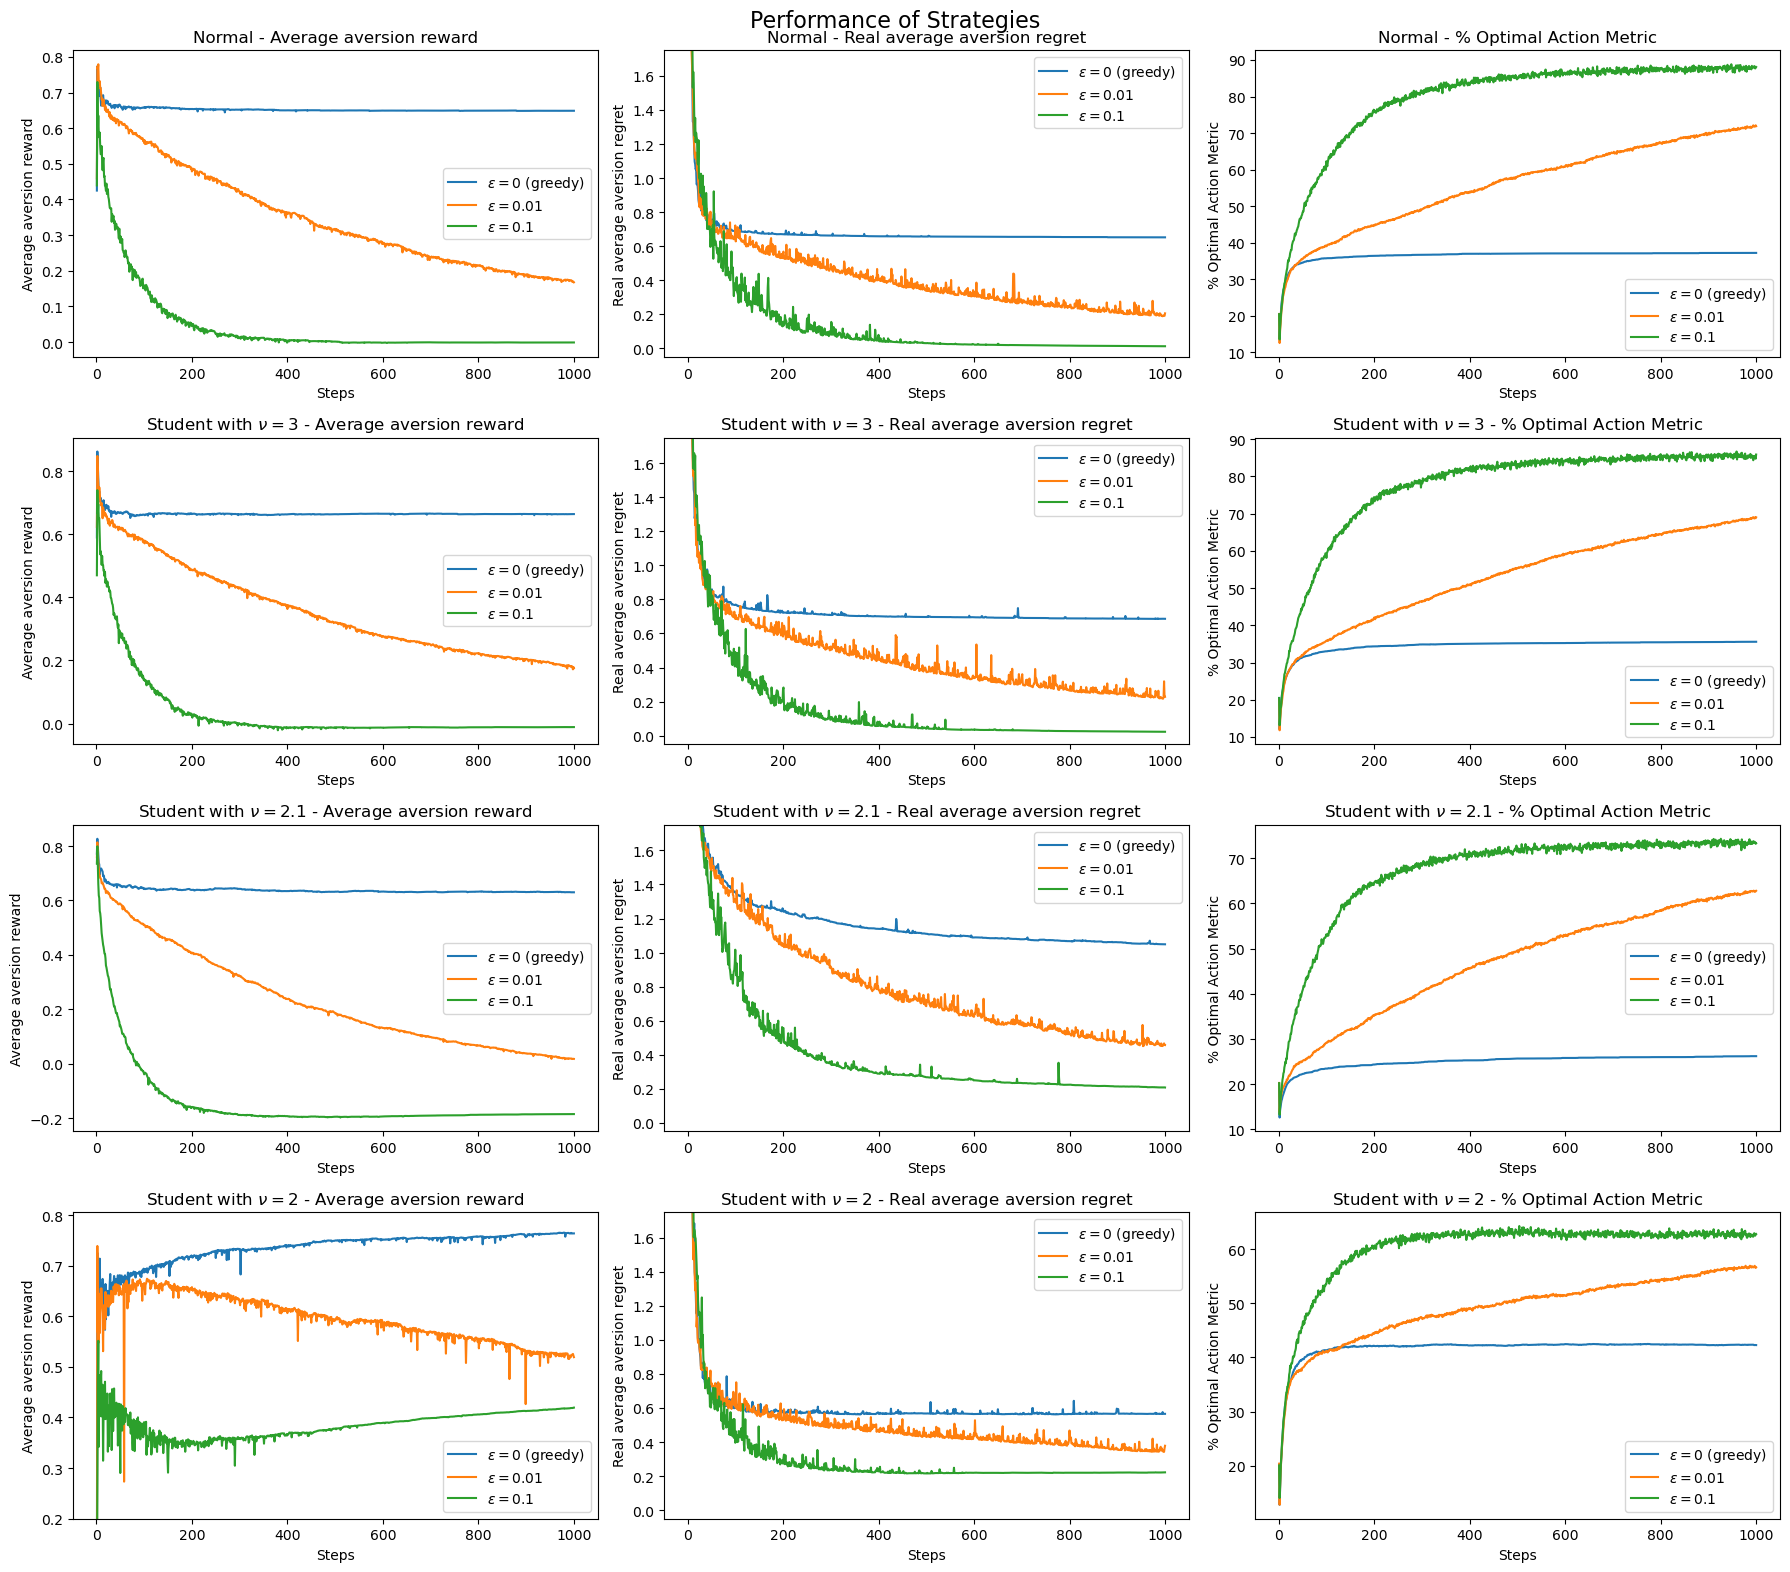
\includegraphics[width=6in]{theory_tester/theory_images/epsilon_greedy/strat_distr.png}
\caption{Зависимость метрик от количества шагов при greedy и $\epsilon$-greedy стратегиях для различных распределений}
\label{fig:epsilon_greedy_strat_distr}
\end{figure}

Как можно видеть из \ref{fig:epsilon_greedy_strat_distr}, для любого распределения добавление случайного выбора улучшает exploration алгоритма, поэтому средние и дисперсии лучше приближаются, и ответ получается более близким к оптимальному. Например, для $t_{\infty}$ и $t_3$ и для $0.1$-greedy алгоритма процент оптимальных действий близок к $90\%$, почти достигая максимально возможного срднего значения в $91\%$. Также заметим, что для $t_{2.1}$ среднее значение сожаления Regret становится отрицательным, в то время как среднее реальное сожаление Regret$_{\text{real}}$ увеличилось на последних шагах до $0.2$ в отличие от $\approx 0$ для $t_3$. Это говорит о том, что алгоритм ``переоценивает'' себя, давая ``якобы'' лучше прибыль, чем оптимальное значения вероятности, из-за чего в реальности прибыль значительно ниже, чем для оптимальной вероятности. \\

Из-за чего это может происходить? Из-за недооценки значения дисперсии. Давайте смоделируем 10000 тестов, в каждом из них возьмем 1000 сэмплов из распределения Стьюдента с $t_{\nu}$ с дипсерсией 1, посчитаем выборочную дисперсию, а затем среди полученных 10000 выборочных дисперсий возьмем медиану. Эта медиана будет приближением медианы распределения выборочной дисперсии $s_{1000}^2$. Построим график зависимости этой медианы от числа степеней свободы при $\nu > 2$. Если бы мы считали выборочное матожидание вместо дисперсии, то ее медиана была бы постоянной и равнялась бы матожиданию $t_{\nu}$. В случае дисперсии все по-другому (см. \ref{fig:median_depend_on_df}):

\begin{figure}[ht!] %!t
\centering
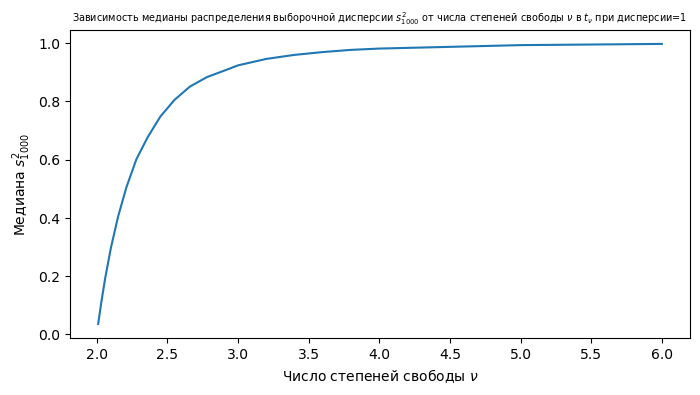
\includegraphics[width=5in]{theory_tester/theory_images/median_depend_on_df.png}
\caption{Зависимость медианы распределения выборочной дисперсии распределения Стьюдента $t_{\nu}$ относительно $\nu$}
\label{fig:median_depend_on_df}
\end{figure}

\begin{figure}[ht!] %!t
\centering
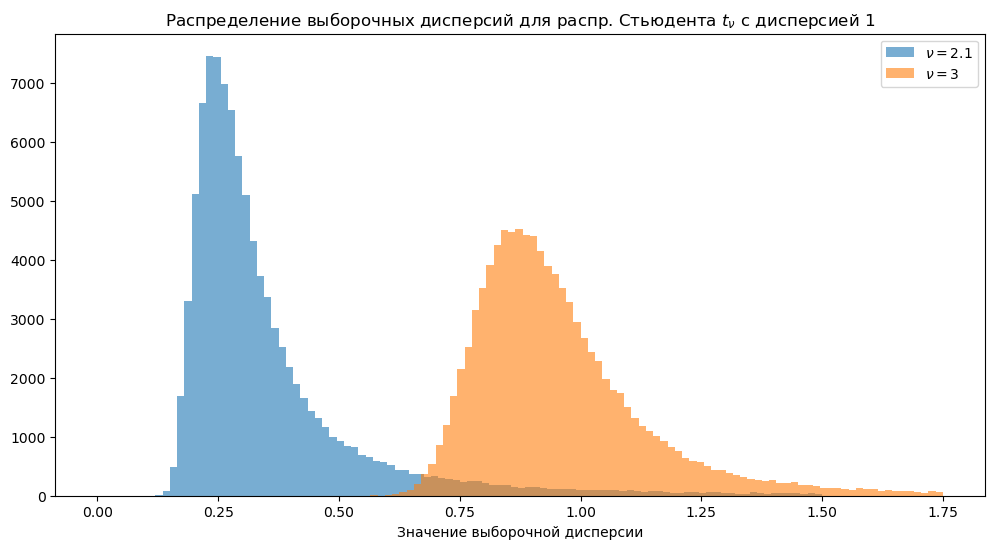
\includegraphics[width=5in]{theory_tester/theory_images/distributions_of_sample_variances.png}
\caption{Распределения выборочных дисперсий для распределений Стьюдента $\nu=2.1$ и $\nu=3$ с дисперсиями 1. Построено на 100000 значениях выборочной дисперсии $s_{1000}^2$}
\label{fig:distributions_of_sample_variances}
\end{figure}

Как можно видеть, медиана стремится к 0 при $\nu \to 2+$. При этом для любого $\nu$ медиана меньше среднего и медиана стремится к 1 при $\nu \to \infty$. В частности, при $\nu=2.1$ медиана примерно равна $0.3$, а при $\nu=3$ -- примерно равна $0.92$ (см. \ref{fig:distributions_of_sample_variances})

Это значит, что в большинстве случаев алгоритм недооценивает реальное значение дисперсии, из-за чего алгоритм склонен недооценивать риски и сосредотачивать деньги в активе с самой большой прибыльностью. А это, в свою очередь, снижает эффективность алгоритма. \label{negative_regret} Кроме того, поскольку дисперсии недооцениваются, то из прибыли вычитается меньшее значение, и потому алгоритм выдает большее значение прибыли, чем для оптимальной вероятности, что дает отрицательное среднее сожаление. \\

Что касается распределения Стьюдента $t_3$, то для него медианное значение дисперсии близко к реальному, поэтому эффект ``переоценки'' почти не проявляется. \\

Как мы выяснили, среди нарисованных на графике стратегий лучше всех работает $0.1$-greedy. Построим для нее график зависимости метрик от коэффциента отвращения для каждого распределения (\ref{fig:aversion_last_5_steps}):

\begin{figure}[h] %!t
\centering
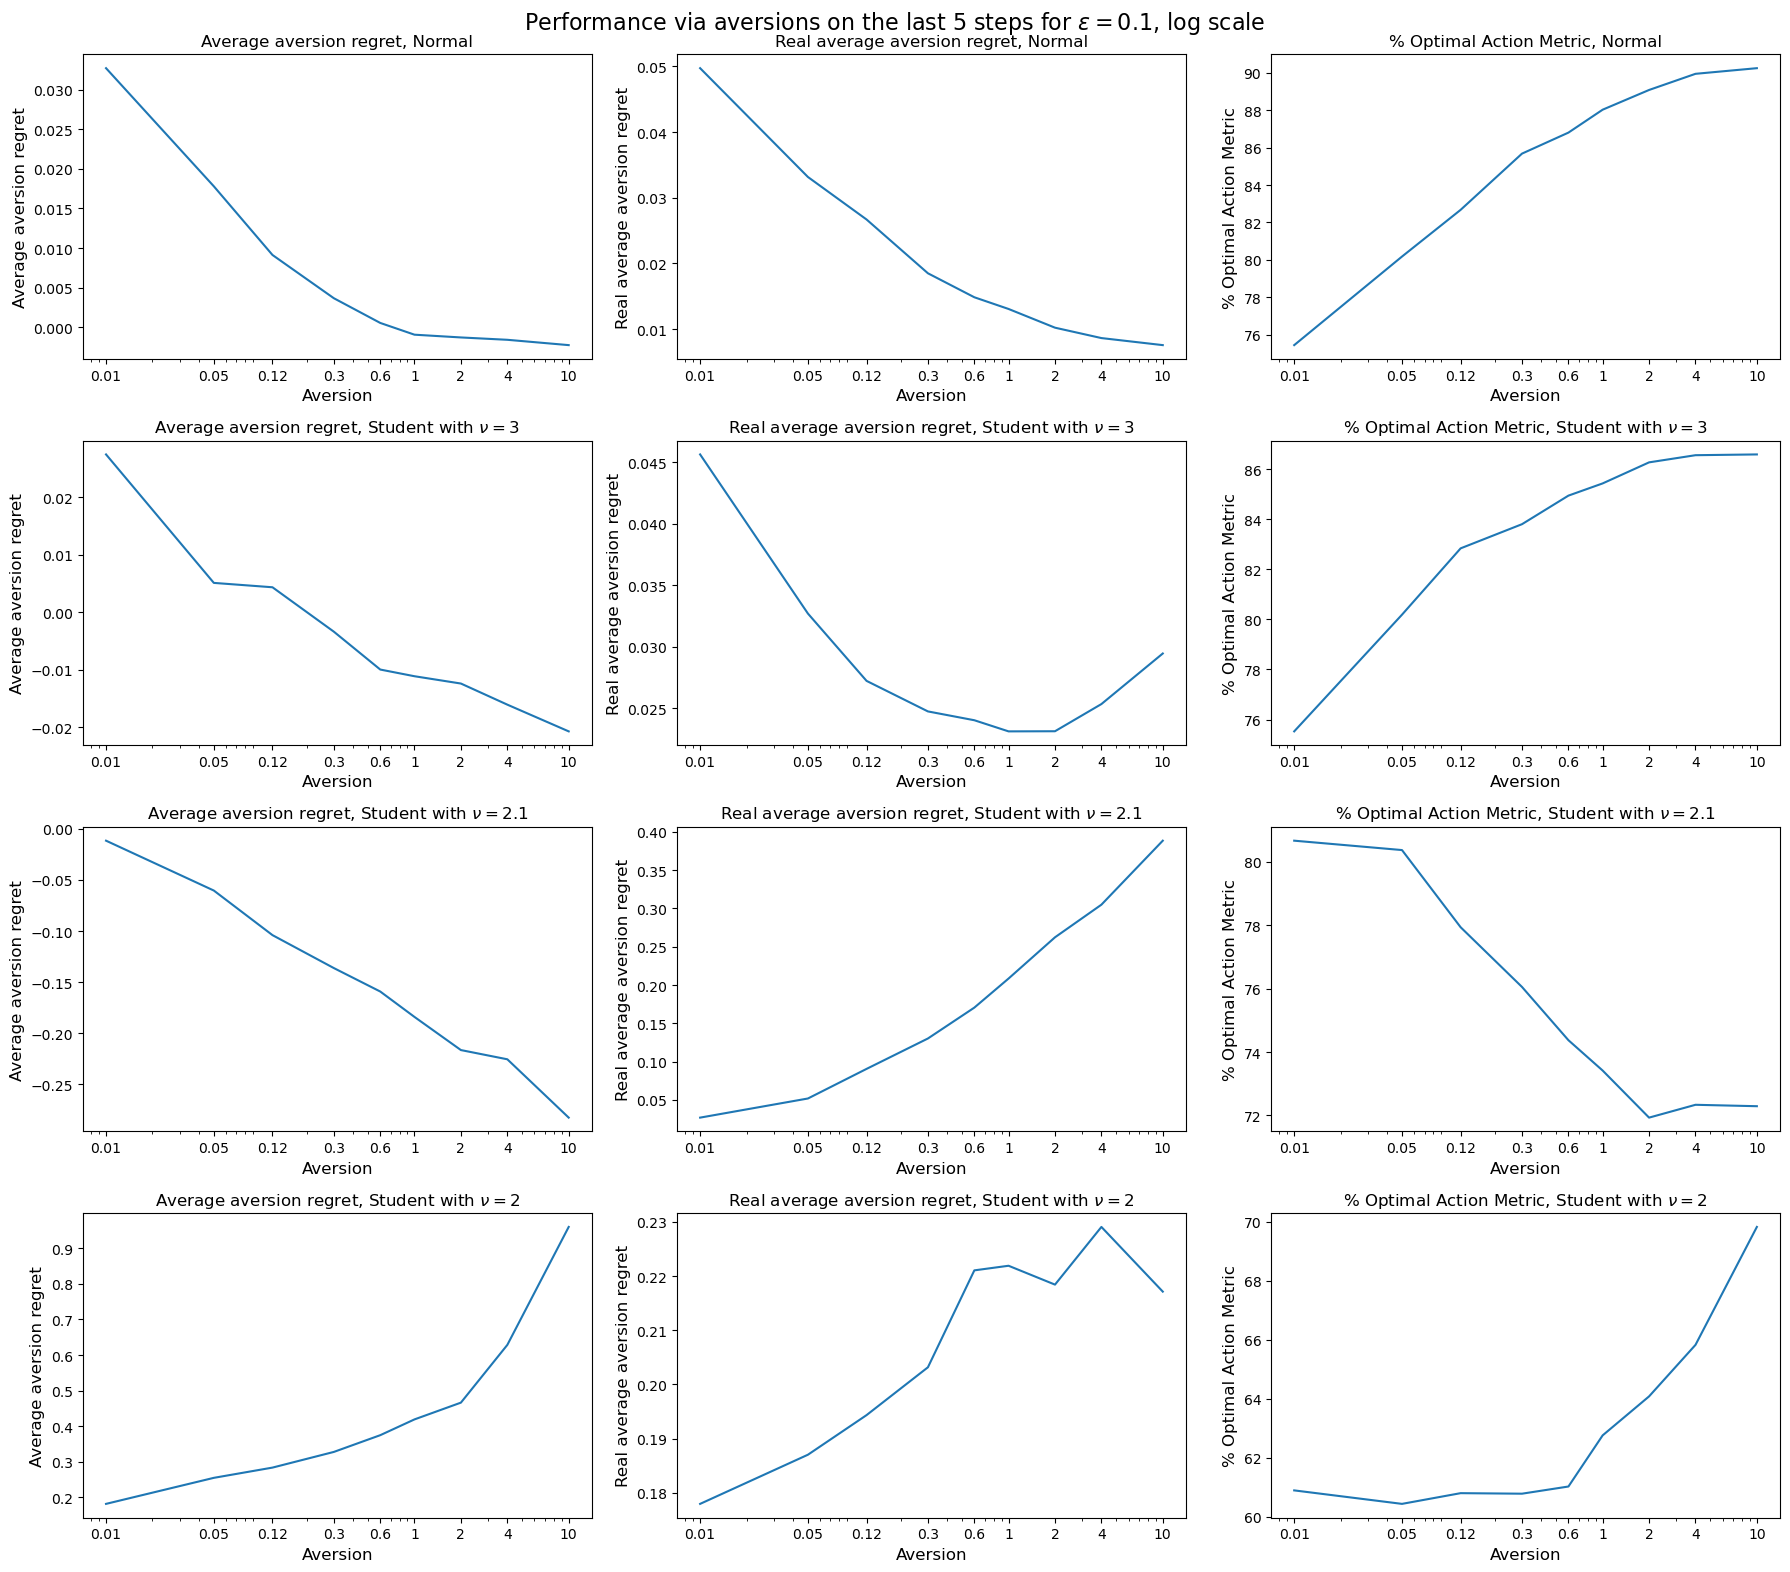
\includegraphics[width=6in]{theory_tester/theory_images/epsilon_greedy/aversion_last_5_steps.png}
\caption{График зависимости метрик от коэффциента отвращения для каждого распределения, усредненное по последним 5 шагам.}
\label{fig:aversion_last_5_steps}
\end{figure}

Как видно из графиков, для любого распределения с $\nu > 2$ при увеличении коэффициента отвращения к риску $\lambda$ метрика Regret уменьшается, и алгоритм переходит от своей недооценки к переоценке. Для $t_3$ и $t_{\infty}$ при увеличении $\lambda$ процент оптимальных действий увеличивается (хотя при $\nu = 3$) Regret$_\text{real}$ имеет минимум. В какой-то момент происходит переход, и для $t_{2.1}$ при уменьшении $\lambda$ точность увеличивается. Для $t_2$ при уменьшении $\lambda$ тоже наблюдается уменьшение Regret$_\text{real}$. \\

Почему при $\lambda \to 0+$ для больших степеней свободы эффективность алгоритма падает? При маленьких $\lambda$ дисперсия почти не учитывается при подсчете формулы, поэтому в оптимальном векторе вероятностей вся вероятность находится в рычаге с наибольшим матожиданием. Возьмем 2 рычага с наибольшим матожиданием $L_1$ и $L_2$ (у $L_1$ матожидание больше). Предположим, что у $L_1$ больше дисперсия, чем у $L_2$ (вероятность этого $\approx 0.5$). Тогда флуктуация получаемых наград у $L_2$ будет больше, чем у $L_1$, а это приводит к тому, что часто случается ситуация, при которой $Q_t(L_1) < Q_t(L_2)$. В таком случае в $91\%$ случаев $0.1$-greedy алгоритм будет выбирать $L_2$, что далеко от оптимального действия нажимать на рычаг $L_1$. При увеличении $\lambda$ этот недостаток нивелируется более равномерным распределением вероятностей по рычагам и потому более частым выбором $L_1$. \\

При $\nu$, близких к 2, описанный выше эффект начинает нивелировать эффект недооценки (преуменьшения) дисперсии: при больших $\lambda$ вероятности более равномерно распределяются по рычагам. Но алгоритм оценивает дисперсию каждого рычага значительно меньше, чем есть на самом деле, поэтому алгоритм старается сильнее концентрировать вероятности в одном рычаге, что дает отличие в векторах вероятностей и итоговое уменьшение эффективности. Далее мы на других графиках увидим, что такое поведение связано именно с преуменьшением дисперсии. \\

Уменьшение метрики Regret на графике для $t_{\infty}$ связано с уменьшением точности алгоритма при уменьшении $\lambda$, а для $t_{3}$ и $t_{2.1}$ это, опять-таки, происходит из-за преуменьшения дисперсии, как было уже сказано ранее \ref{negative_regret}. \\

\begin{figure}[h] %!t
\centering
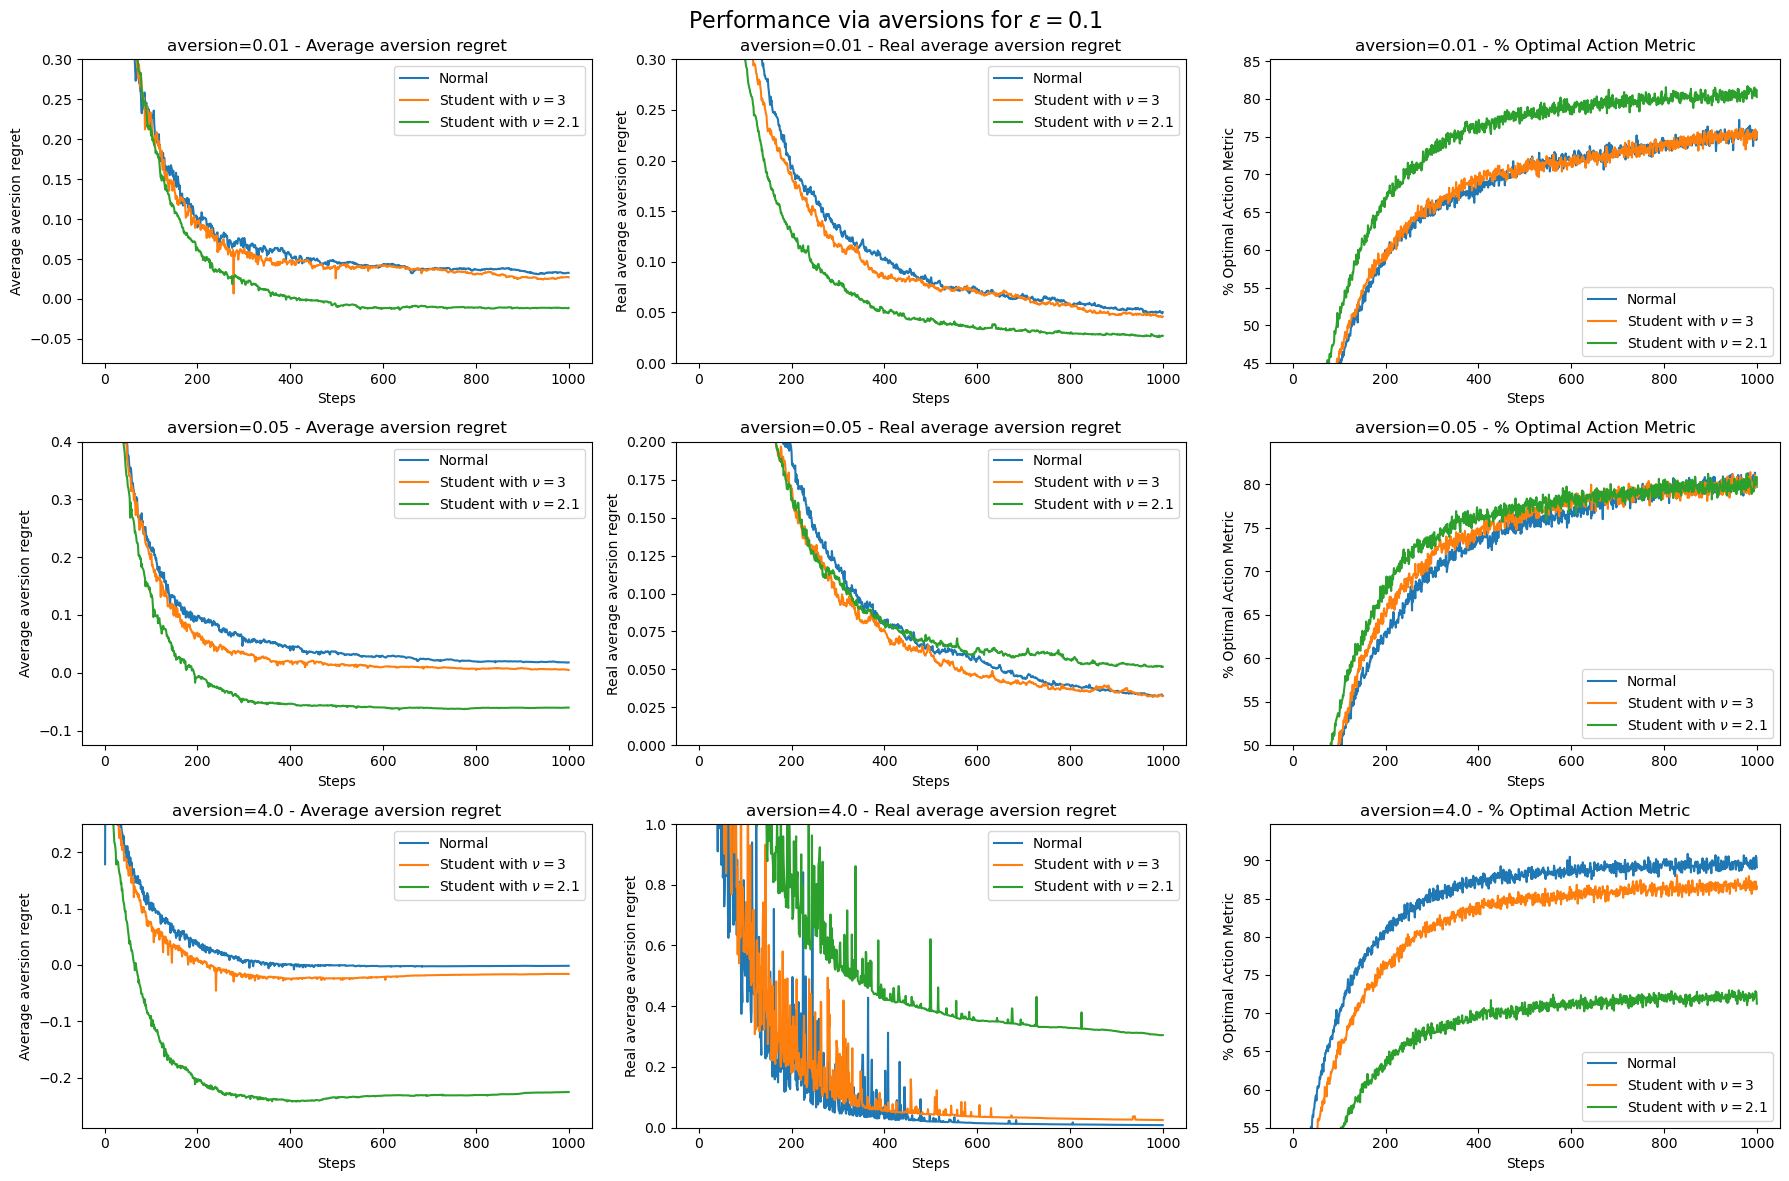
\includegraphics[width=6in]{theory_tester/theory_images/epsilon_greedy/aversion_selected_aversions.png}
\caption{Графики зависимости метрик от количества шагов для каждого коэффициента отвращения.}
\label{fig:eps_greedy_aversion_selected_aversions}
\end{figure}

Что еще интересно, так это то, что при маленьком $\lambda$ эффективность для $t_{2.1}$ выше, чем для $t_3$ и $t_{\infty}$, но приувеличении коэффициента отвращения ситуация меняется, и  для $t_{2.1}$ метрики становятся хуже, чем для $t_3$ и $t_{\infty}$ (см. \ref{fig:eps_greedy_aversion_selected_aversions}). При больших $\lambda$, как было замечено выше, это связано с недооценкой дисперсии. При маленьких $\lambda$ дисперсия уже не играет при нахождении вероятностей никакой роли. Так в чем же дело? Предполагаю, что дело в более тяжелых хвостах у $t_{2.1}$: при нажатии на рычаг у $t_{2.1}$ среднее меняется сильнее, чем у $t_3$ и $t_{\infty}$, что приводит к тому, что каждый из рычагов для $t_{2.1}$ в среднем выбирается чаще, что, в свою очередь, частично решает проблему с плохим приближением средних для двух рычагов с наибольшим средним и способствует тому, чтобы алгоритм ставил вероятность выбора рычага с наибольшим средним с близкой к 1 вероятностью.

\subsection{Коррекция выборочной дисперсии}\label{sec:correction_eps_greedy}

Итак, как мы выяснили, в связи со смещенной влево (относительно матожидания) медианой у выборочного среднего $s_n^2$ алгоритм в большинстве случаев недооценивает реальную димперсию распределения. Предположим, что алгоритму откуда-то стало известно семейство распределений, откуда генерируются активы. Модифицируем алгоритм, чтобы исправить описанную проблему. \\

Пусть алгоритм будет домножать выборочную дисперсию каждого распределения на определенную константу. Мы хотим домножить на такое число, чтобы произведение с большой вероятностью было близко к реальной дисперсии. Понятно, что при увеличении дисперсии в $\alpha$ раз распределение выборочной дисперсии тоже ``растягивается'' в $\alpha$ раз. Рассмотрим единичную дисперсию. Возьмем такие 2 варианта константы:
\begin{enumerate}
    \item $c_m = \frac{1}{m}$, где $m$ -- медиана распределения выборочной дисперсии $s_{1000}^2$ распределения с дисперсией $\sigma^2=1$ -- median correction.
    \item $c_{\mu} = \frac{1}{\mu}$, где $\mu$ -- мода распределения выборочной дисперсии $s_{1000}^2$ распределения с дисперсией $\sigma^2=1$ -- mode correction.
\end{enumerate}
Обе константы можно посчитать, сгенерировав $k$ выборок из $1000$ наград, где $k$ достаточно большое, посчитав в каждой выборке выборочную дисперсию, а затем среди полученных $k$ значений либо взять медиану, либо, взяв дискретизацию значений, посчитать среди них наиболее часто встречающееся. Взяв $k=5\cdot 10^{5}$ и дискретизацию по трем знакам после запятой, для $t_{2.1}$ были получены следующие значения: $c_m = 3.37269, \: c_{\mu} = 4.03226$. Подставим эти значения в алгоритм $\epsilon$-greedy с $\epsilon = 0.1$ и распределением $t_{2.1}$. При подсчете сожаления будем подставлять исправленную выборочную дисперсию. Сравним полученный результат с $0.1$-greedy алгоритмом без корректировки дисперсии.

\begin{figure}[h] %!t
\centering
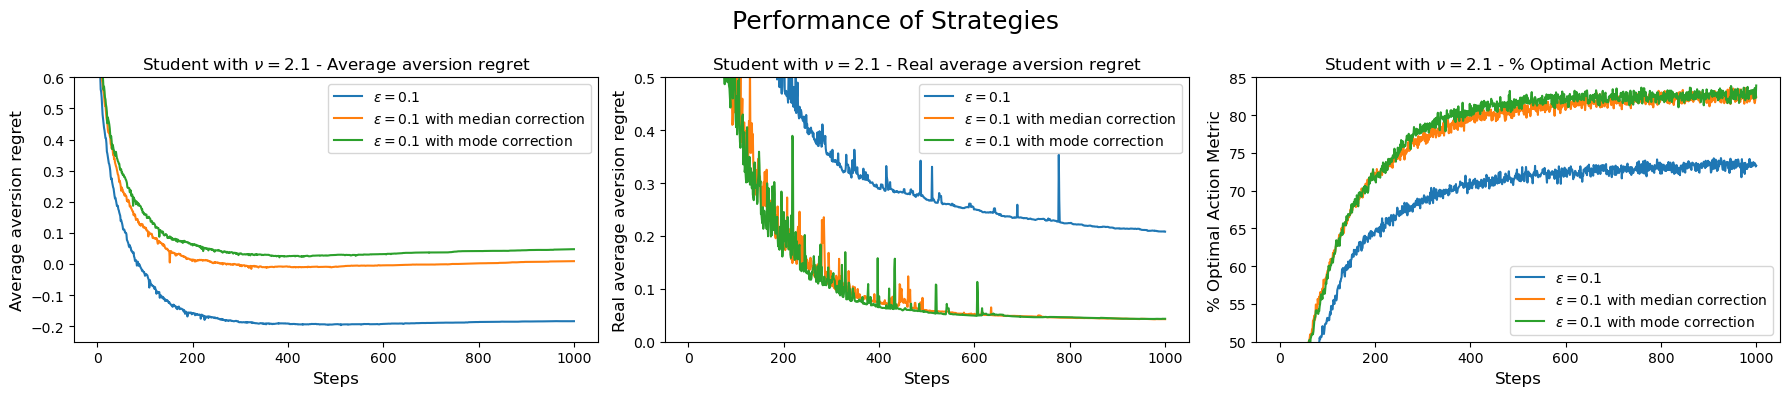
\includegraphics[width=6in]{theory_tester/theory_images/correction_variance/strat_distr.png}
\caption{Графики зависимости метрик от количества шагов для $t_{2.1}$ и стратегий с корректировкой выборочной дисперсии. Рассмотрена корректировка с помощью доиножения на $c_m, \: c_{\mu}$ и без домножения (обычный $\epsilon$-greedy.)}
\label{fig:correction_aversion_strat_distr}
\end{figure}

\begin{figure}[h] %!t
\centering
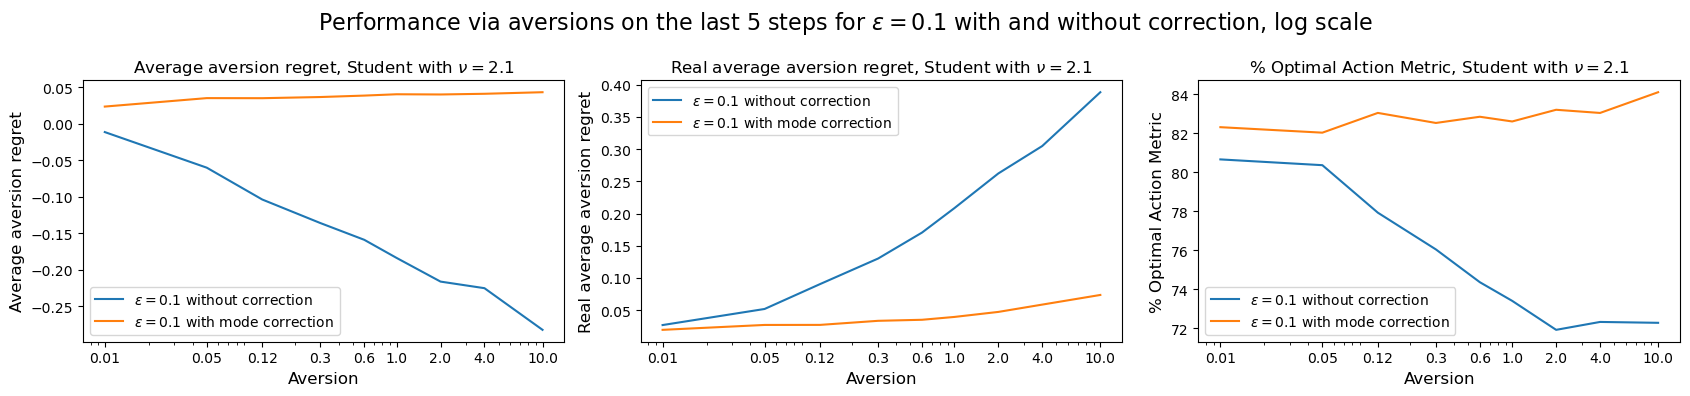
\includegraphics[width=6in]{theory_tester/theory_images/correction_variance/aversions_last_5_steps.png}
\caption{Графики зависимости метрик от коэффициента отвращения для $t_{2.1}$ и стратегий с корректировкой выборочной дисперсии. Рассмотрена корректировка с помощью доиножения на $c_{\mu}$ и без домножения (обычный $\epsilon$-greedy.)}
\label{fig:correction_aversion_strat_distr}
\end{figure}

\begin{figure}[h] %!t
\centering
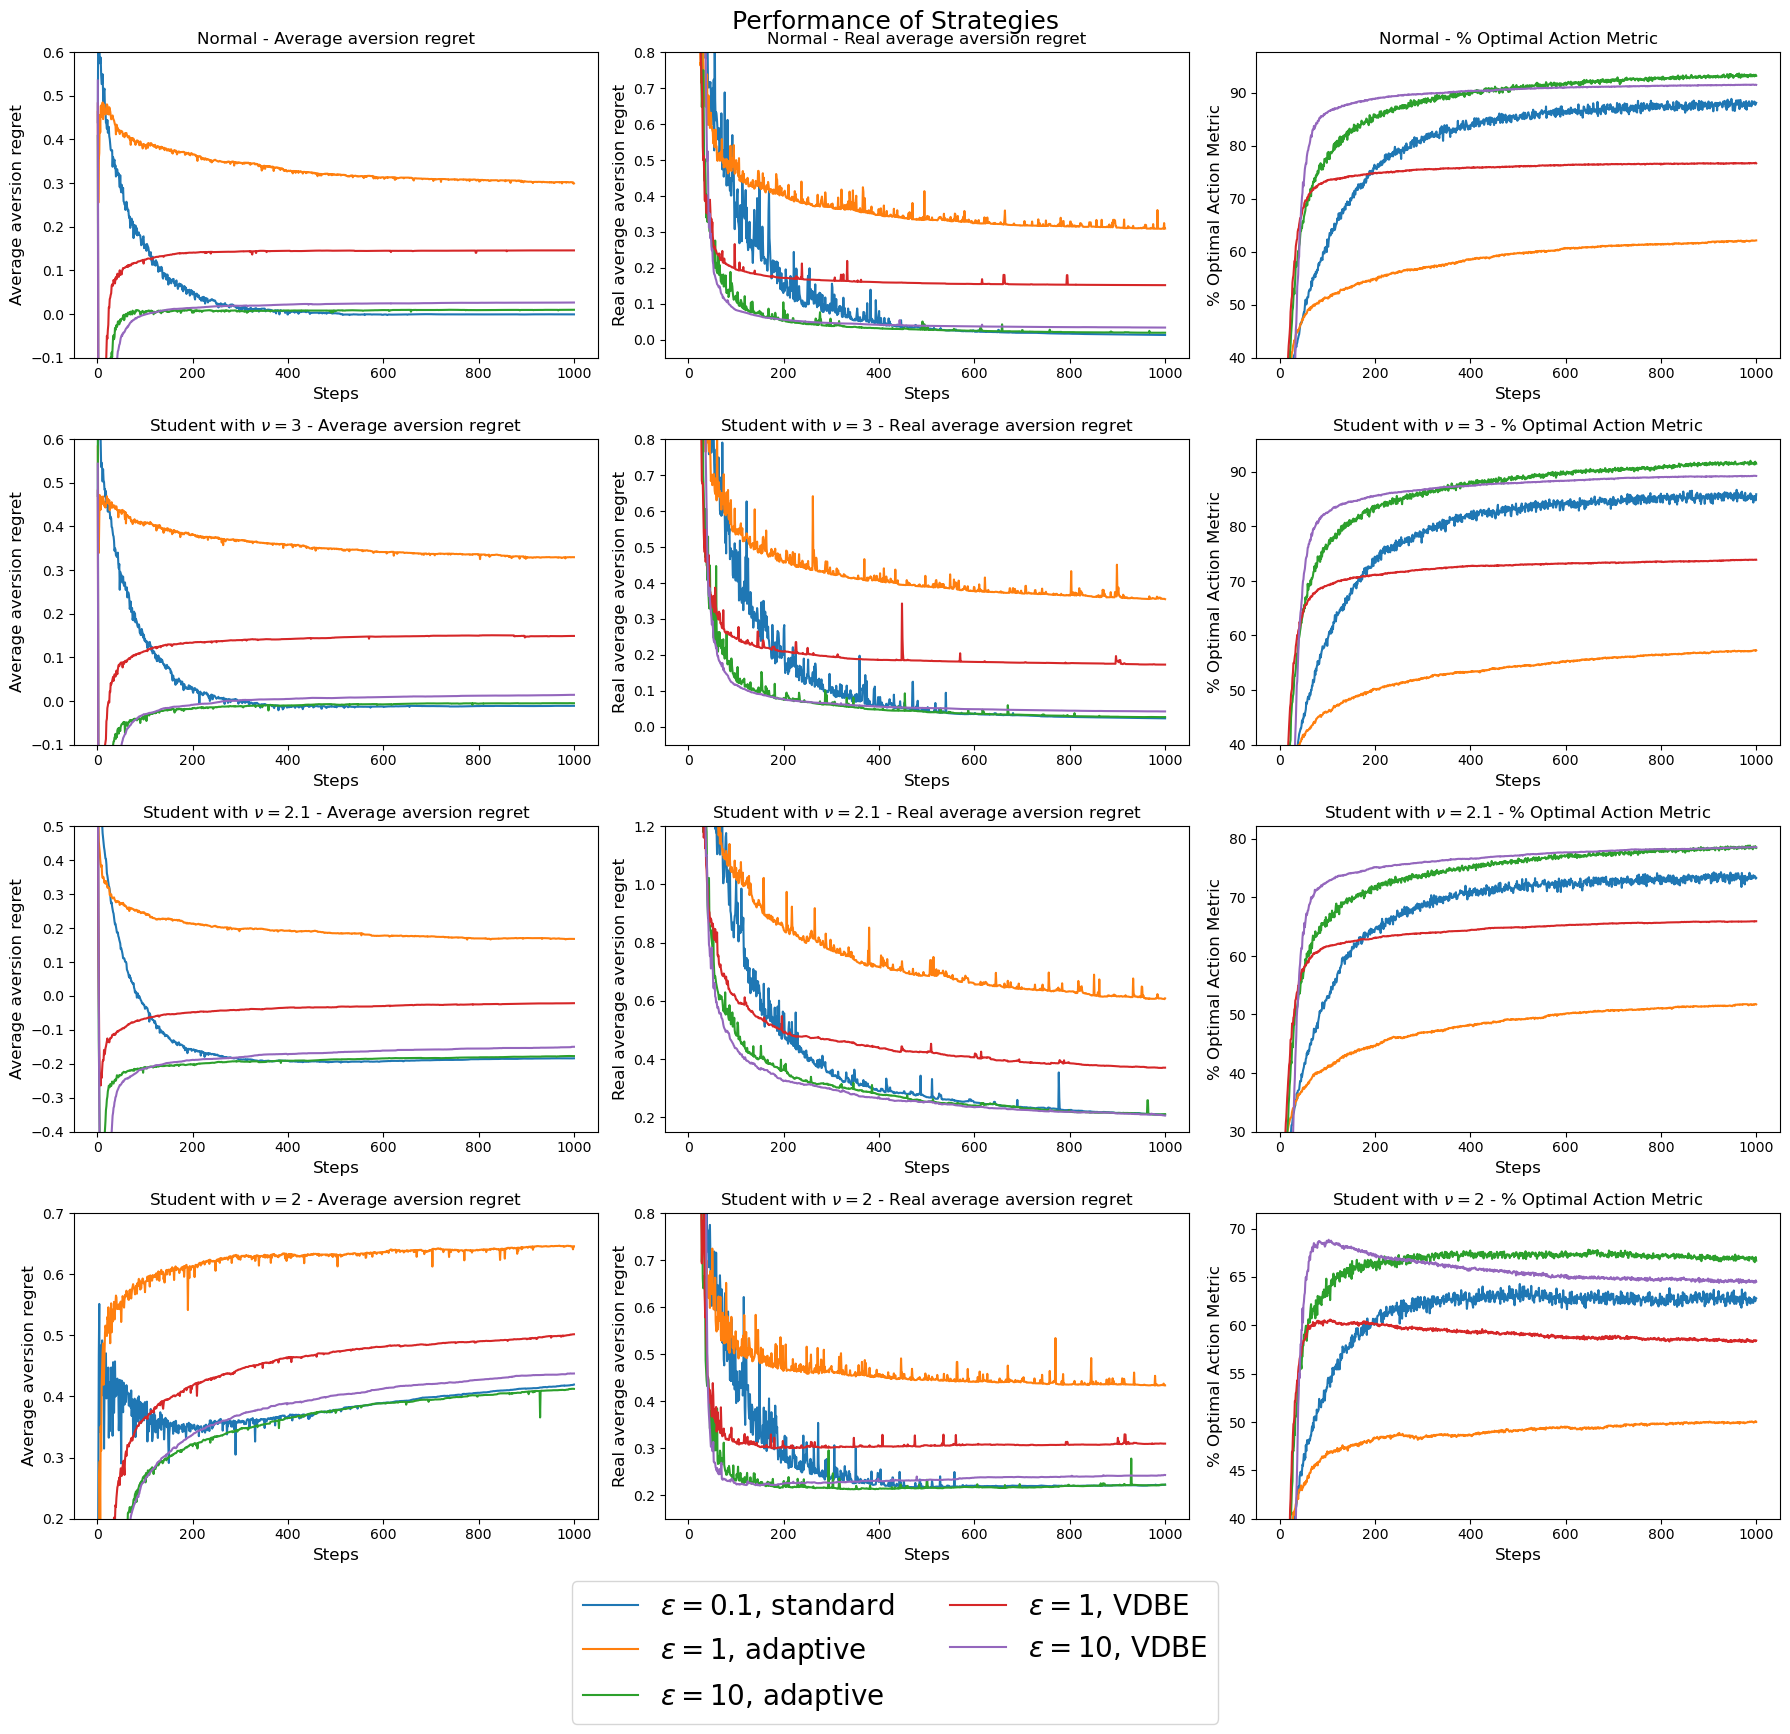
\includegraphics[width=6in]{theory_tester/theory_images/adaptive_epsilon/one_distr.png}
\caption{Зависимость метрик от количества шагов при $0.1$-greedy, adaptive-$\epsilon$ и VDBE стратегиях для различных распределений}
\label{fig:adaptive_eps_strat_distr}
\end{figure}

Как можно видеть, коррекция дисперсии значительно улучшает значения метрик. В частности, метрика Regret для стратегий с увеличением дисперсий не опускается ниже 0. Но процент оптимальных действий достигает максимального значения в примерно $85\%$, что меньше $90\%$, то есть у этих стратегий, при всех их преимуществах, устранены не все недостатки. Хотя у коррекций с помощью медианы и моды примерно одинаковые результаты, последняя все-таки незначительно лучше.

Оценим изменение значения метрик при различных коэффициентах отвращения для обычной $0.1$-greedy стратегии и для $0.1$-greedy стратегии с коррекцией с помощью моды.

Увеличение выборочной дисперсии практически устраняет с увеличением $\lambda$ ухудшение метрик Regret и Regret$_\text{real}$ и полностью устраняет уменьшение процента оптимальных действий. При этом в случае с процентом оптимальных действий можно наблюдать некоторое уменьшение метрик при $\lambda \to 0$, то есть начинает проявляться эффект неточности для двух рычагов с наибольшим матожмданием. В случае же Regret полномтью пропала переоценка стратегией самой себя. В целом же значения метрик для коррекции с помощью $c_{\mu}$ лучше, чем без коррекции при всех $\lambda$. \\

Хотя домножение дисперсии значительно улучшает эффективность стратегии, в реальной жизни это малоприменимо -- зачастую нам неизвестно число степеней свободы у распределения прибыли актива. Угадать константу, на которую нужно домножить, тоже не представляется возможным, поскольку значение медианы при $\nu > 2$ меняется от 0 до 1, и поэтому $c_m$ (и $c_{\mu}$) меняются от 1 до $\infty$ (см. \ref{fig:median_depend_on_df}).

\subsection{Адаптивный $\epsilon$-greedy}

Вернемся к стратегиям без коррекции дисперсии. Для стратегий с адаптивным $\epsilon$ получились следующие результаты (см. \ref{fig:adaptive_eps_strat_distr}):

Для всех распределений наилучшие результаты показали стратегии с начальным $\epsilon=10$. Это объясняется тем, что на начальных шагах у этих стратегий происходит фаза exploration, во время которой вероятности нажатий на рычаги распределены почти равномерно. Из-за этого дисперсии и матожидания приближаются более точно. Для $t_3$ и $t_{\infty}$ наилучший результат показала адаптивная $\epsilon$-greedy стратегия с $\epsilon=10$. Чуть хуже результаты у VDBE с $\epsilon=10$. Для $t_{2.1}$ эти стратегии показали примерно одинаковый результат. В отличие от $\epsilon$-greedy, адаптивные стратегии склонны к сильной переоценке своих результатов на начальных шагах (в то время как $\epsilon$-greedy, наоборот, недооценивает себя). ПОЧЕМУ? НАПИШИ. \\

Поскольку стратегии с $\epsilon=10$ показали наилучший результат, посмотрим на изменение метрик для этих стратегий при различных коэффициентах отвращения:

\begin{figure}[ht!] %!t
\centering
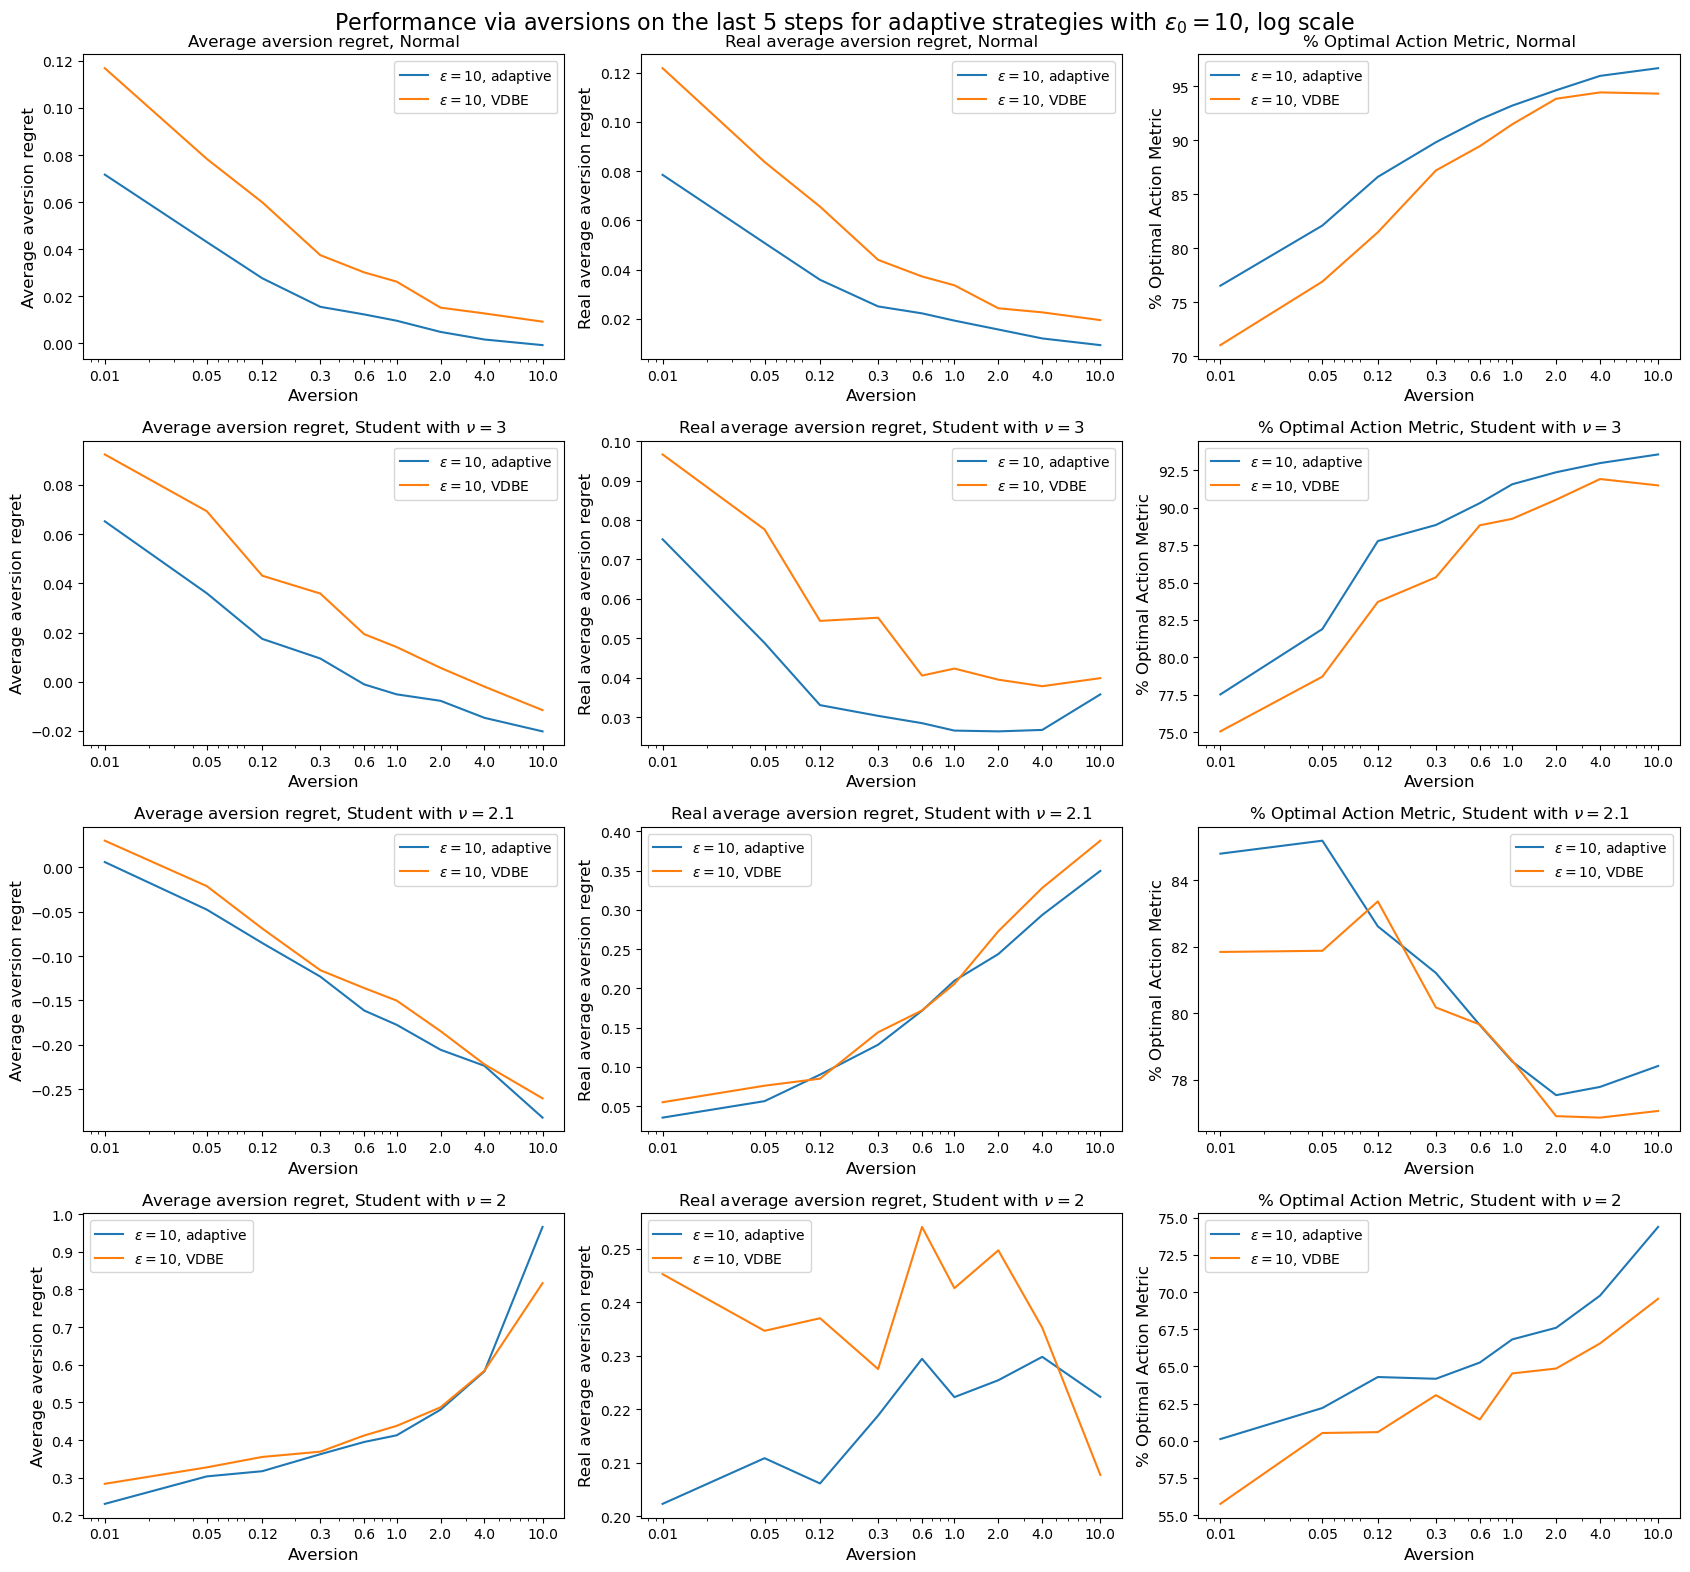
\includegraphics[width=6in]{theory_tester/theory_images/adaptive_epsilon/aversion_last_5_steps.png}
\caption{Графики зависимости метрик от коэффициента отвращения для $t_{2.1}$ и стратегий adaptive-$\epsilon$ и VDBE с $\epsilon=10$.}
\label{fig:adaptive_eps_last_5_steps}
\end{figure}

Как видно из \ref{fig:adaptive_eps_last_5_steps}, тенденция изменения метрик с изменением $\lambda$ схожа с таковой у $\epsilon$-greedy стратегии. Также стратегия adaptive-$\epsilon$ показывает себя лучше, чем VDBE. Однако VDBE обладает бОльшим потенциалом, поскольку позволяет настраивать дополнительные параметры -- температуру $\tau$ и шаг обновления $\delta$. Изучение поведения VDBE при различных параметрах $\epsilon$, $\tau$ и $\delta$ может быть интересной темой для дальнейших исследований.

\subsection{Позитивная инициализация}

Как было замечено ранее, для $t_{\nu}$ с $\nu > 2$ в обычной задаче о многоруких бандитах позитивная инициализация с постоянным step-size показывает результат лучше, чем $\epsilon$-greedy, при этом обучаясь до наибольших значений своих метрик за горяздо меньшее время. При этом у позитивной инициализации наблюдался эффект переобучения. Попробуем посмотреть на результаты этой стратегии в задаче с присутствием неприятия к риску.

\begin{figure}[ht!] %!t
\centering
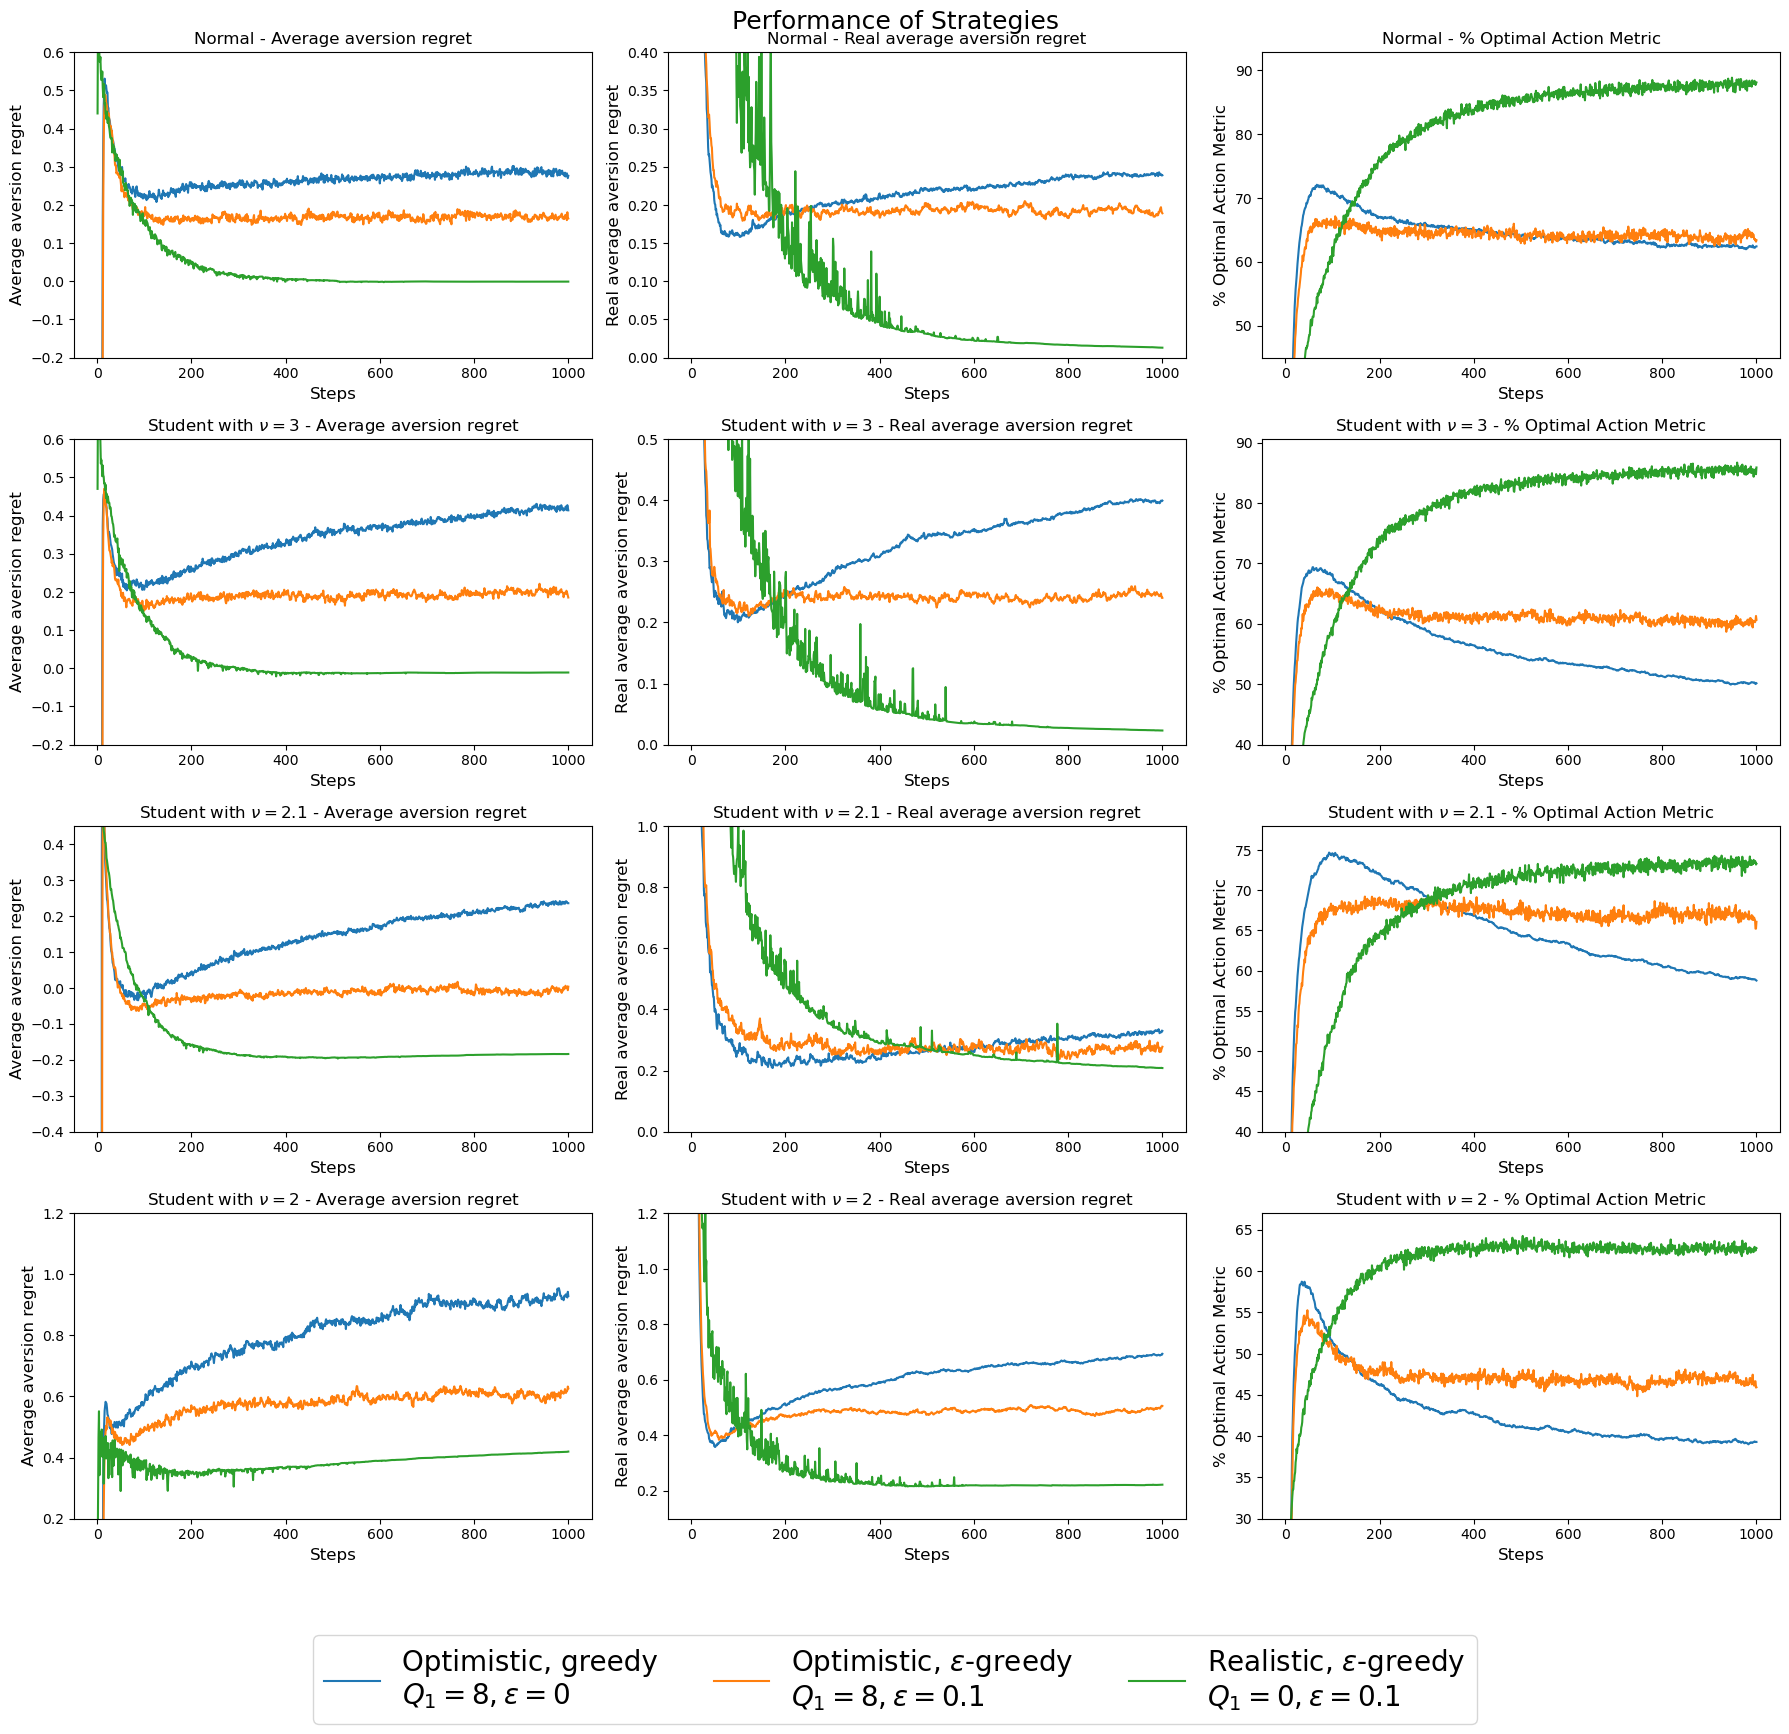
\includegraphics[width=6in]{theory_tester/theory_images/positive_init/one_distr.png}
\caption{Зависимость метрик для различных распределений от количества шагов при стратегиях с позитивной инициализацией, постоянным step-size и $\epsilon=0$ или $\epsilon=0.1$, а также при $0.1$-greedy стратегии}
\label{fig:positive_init_one_distr}
\end{figure}

Так же, как и в обычной задаче о многоруких бандитах, при позитивной инициализации наблюдается эффект переобучения. Однако в задаче о многоруких бандитах с учетом неприятия к риску эта стратегия превосходит $\epsilon$-greedy только для $t_{2.1}$. Несомненныи плюсом является то, что для достижения наилучших значений метрик позитивной инициализации понадобилось намного меньше шагов, чем $\epsilon$-greedy -- около 100 против 1000. Что еще интересно, так это то, что при $\lambda \to 2+$ наилучший процент оптимальных действий для жадной стратегии с позитивной инициализацией увеличивается (см. \ref{fig:positive_init_one_strat_positive_greedy}).

\begin{figure}[ht!] %!t
\centering
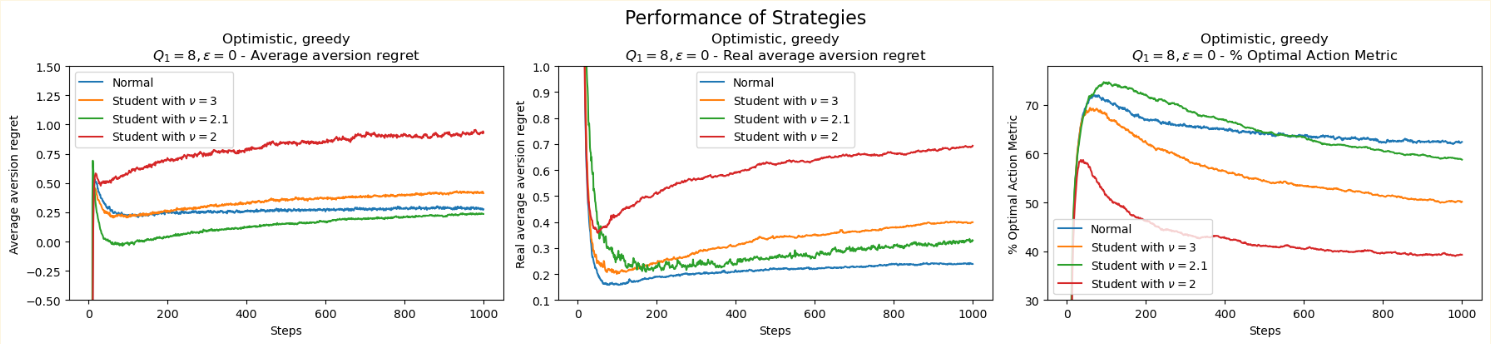
\includegraphics[width=6in]{theory_tester/theory_images/positive_init/one_strat_positive_greedy.png}
\caption{Зависимость метрик для различных распределений от количества шагов для жадной стратегии с позитивной инициализацией и постоянным step-size}
\label{fig:positive_init_one_strat_positive_greedy}
\end{figure}

\subsection{UCB}

В UCB изменению подверглось только выборочное матожидание, выборочную дисперсию изменения не тронули. Неудивительно, что UCB лишь незначительно улучшил результат для $t_{2.1}$, в остальных случаях показав ухудшение относително $0.1$-greedy (см. \ref{fig:ucb_compare_ucb_and_eps_greedy}).

\begin{figure}[ht!] %!t
\centering
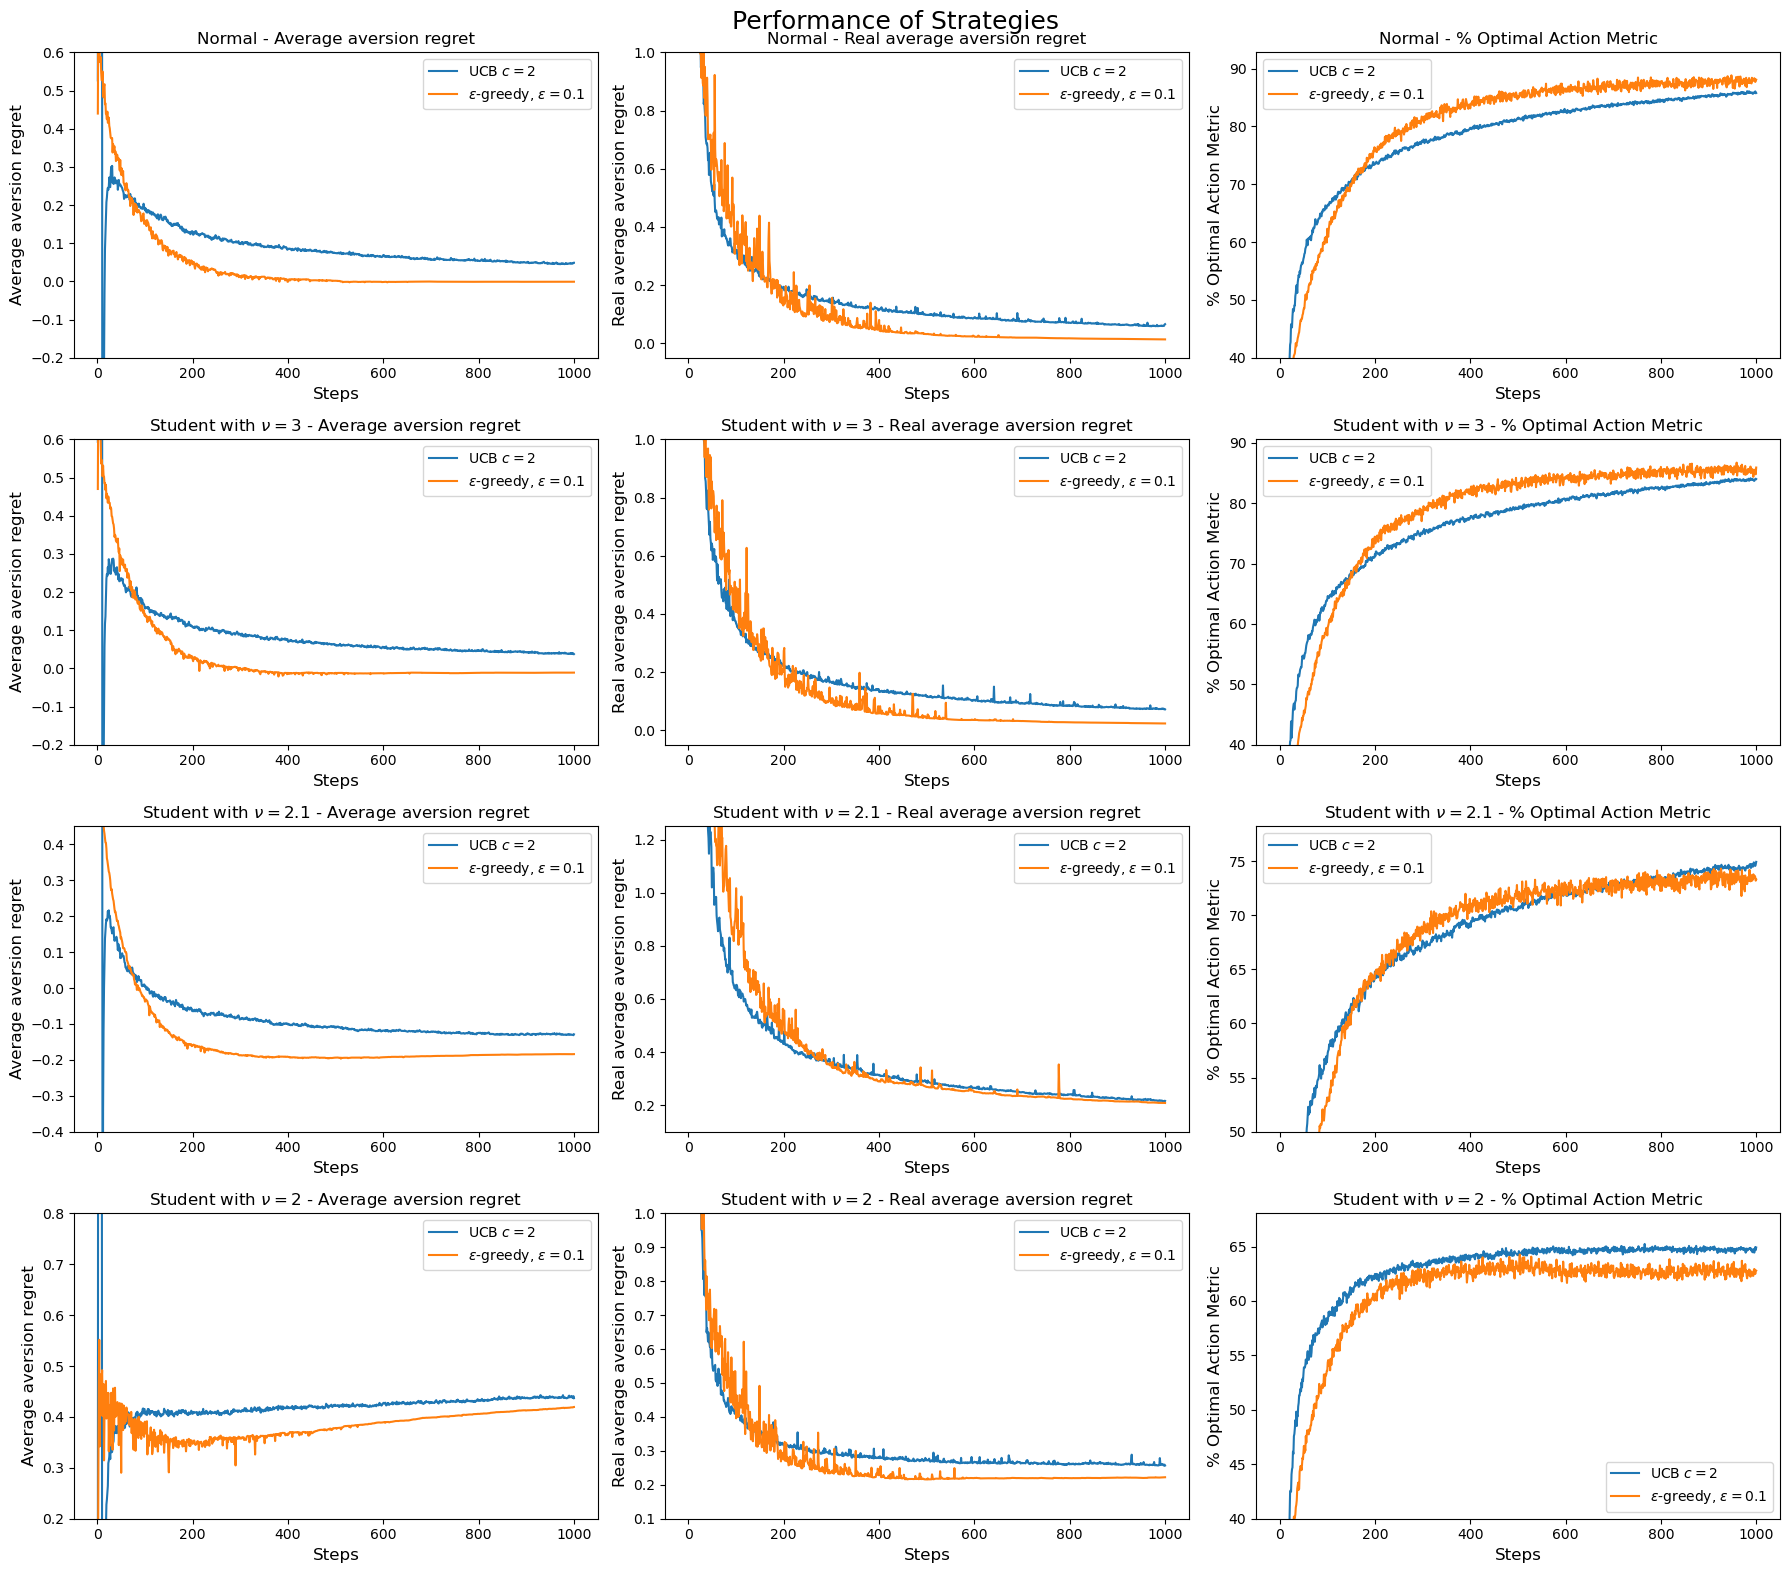
\includegraphics[width=6in]{theory_tester/theory_images/UCB/compare_ucb_and_eps_greedy.png}
\caption{Зависимость метрик для различных распределений от количества шагов для UCB с $c=2$ и $0.1$-greedy}
\label{fig:ucb_compare_ucb_and_eps_greedy}
\end{figure}

\begin{figure}[ht!] %!t
\centering
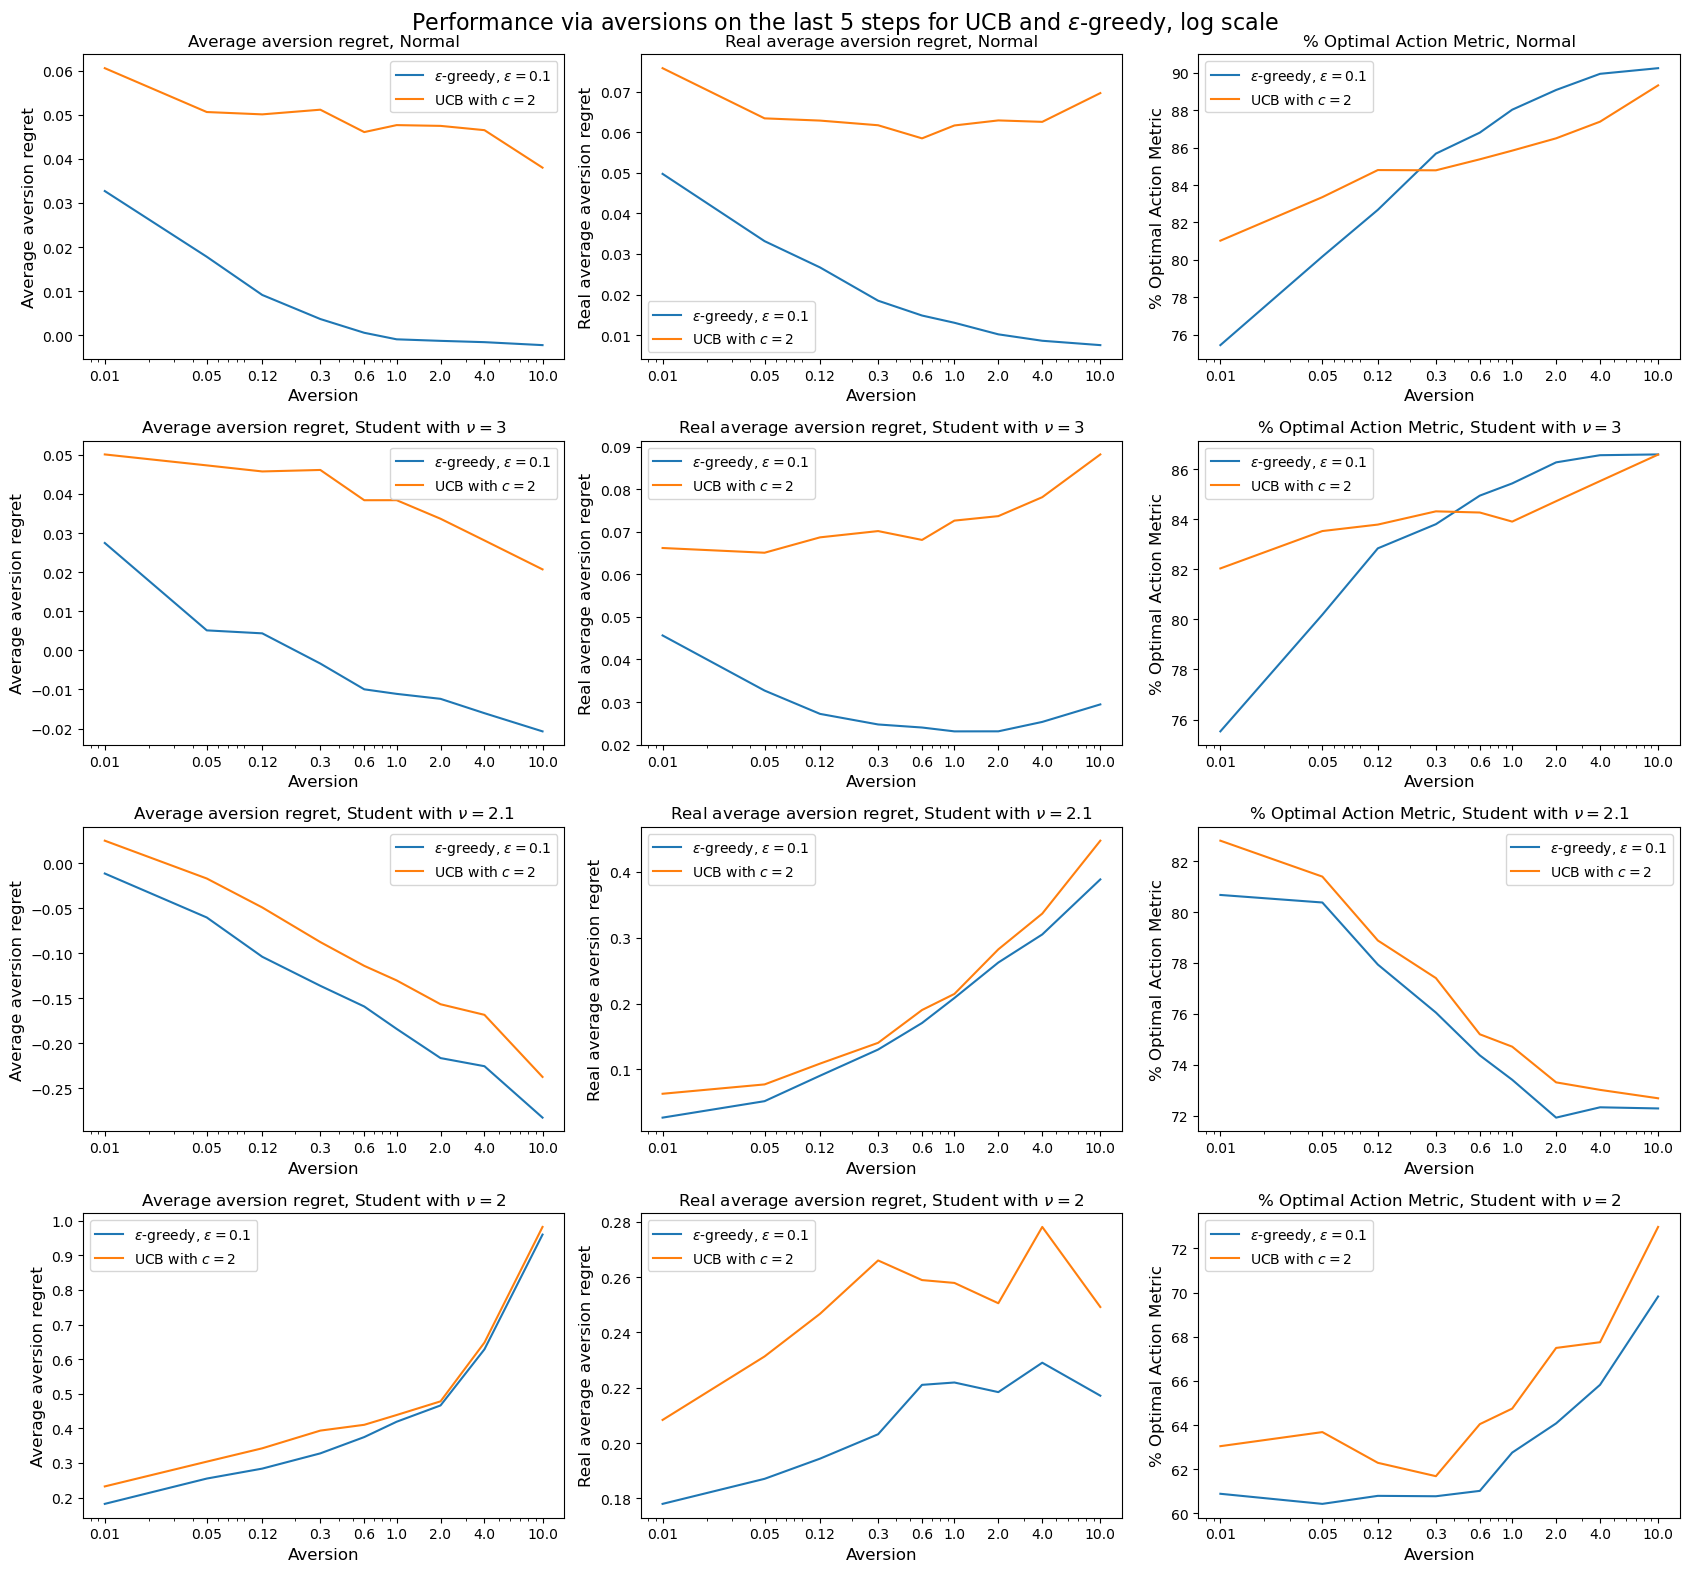
\includegraphics[width=6in]{theory_tester/theory_images/UCB/compare_ucb_for_different_aversions.png}
\caption{Графики зависимости метрик от коэффициента отвращения для различных распределений и стратегий UCB с $c=2$ и $\epsilon$-greedy}
\label{fig:ucb_compare_ucb_for_different_aversions}
\end{figure}

Однако, что интересно (\ref{fig:ucb_compare_ucb_for_different_aversions}), во-первых, для $t_{2.1}$ при любом $\lambda$ у UCB процент оптимальных действий выше, чем у $\epsilon$-greedy. Во-вторых, при маленьких $\lambda$ процент оптимальных действий у UCB выше, чем у $\epsilon$-greedy. Это объясняется тем, что прибавка вида $c\sqrt{\frac{\log t}{N_t(a)}}$ позволяет двум рычагам с наибольшими матожиданиями прожаться большее число раз, что дает лучшее приближение и, как следствие, лучший процент оптимальных действий. В-третьих, при всех $t_{\nu}$ и всех $\lambda$ значение метрики Regret$_\text{real}$ у UCB выше, чем у $\epsilon$-greedy (при том, что в некоторых случаях процент оптимальных действий лучше). После измерения дисперсий метрик оказалось, что дисперсии Regret$_\text{real}$ для UCB и $\epsilon$-greedy одинаковы. Такое странное поведение метрик можно объяснить большей рискованностью UCB: хотя UCB в среднем подбирается ближе к оптимальной точке, чем $\epsilon$-greedy, UCB подбирается к этой точке с более ``крутой'' стороны, что дает болеесильное падение результата. По этой причине, хотя стратегия имеет право на существование, все же она не подходит для реальной жизни.

\subsection{Gradient bandits}

ДОПИШИ!

\bibliographystyle{alpha}
\bibliography{theory_tester/theory_tester}

\end{document}